\documentclass[aspectratio=169]{beamer}

\usetheme{Boadilla}

\usepackage{tikz}
\usetikzlibrary{positioning, calc, arrows.meta, shapes.geometric, patterns}
\usepackage{amsmath}
\usepackage{booktabs}
\usepackage{xcolor}
\usepackage{graphicx}
\graphicspath{{figures/}}

% ── Color palette ─────────────────────────────────────────────────────────────
\definecolor{TechBlue}{RGB}{0, 50, 100}
\definecolor{TechMid}{RGB}{30, 100, 180}
\definecolor{matA}{RGB}{180, 50, 50}       % expensive matrix
\definecolor{matB}{RGB}{40, 130, 70}       % cheap matrix
\definecolor{matC}{RGB}{40, 70, 180}       % output matrix
\definecolor{cacheYellow}{RGB}{210, 150, 0}

\setbeamercolor{title}{fg=white, bg=TechBlue}
\setbeamercolor{frametitle}{fg=white, bg=TechBlue}
\setbeamercolor{structure}{fg=TechBlue}
\setbeamercolor{block title}{fg=white, bg=TechMid}
\setbeamercolor{block body}{bg=TechMid!10}
\setbeamerfont{title}{size=\large, series=\bfseries}
\setbeamerfont{frametitle}{series=\bfseries}
\setbeamertemplate{navigation symbols}{}

% ── Title metadata ─────────────────────────────────────────────────────────────
\title[Mixed-Precision MatMul Tiling]{%
  Cache-Optimal Tiling for\\[4pt]
  Mixed-Precision Matrix Multiplication%
}
\author[Mkhitaryan \textbullet{} Ginzburg]{%
  Areg Mkhitaryan \and Regev Ginzburg%
}
\institute[Technion]{%
  Technion -- Israel Institute of Technology\\[4pt]
  {\small Supervisor: Alon Amid}%
}
\date{}

% ──────────────────────────────────────────────────────────────────────────────
\begin{document}

\begin{frame}[plain]
  \titlepage
\end{frame}

% ==============================================================================
\section{The Problem}
% ==============================================================================

% ── Slide 1: the computation ──────────────────────────────────────────────────
\begin{frame}{Matrix Multiplication with Mixed Precision}

  \begin{columns}[c]

    % Left: visual
    \begin{column}{0.52\textwidth}
      \centering
      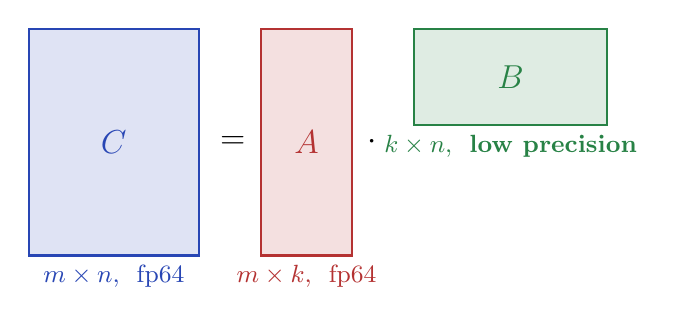
\begin{tikzpicture}[scale=0.72]
        % C
        \fill[matC!15] (0,0) rectangle (3.0, 4.0);
        \draw[matC, thick] (0,0) rectangle (3.0, 4.0);
        \node[matC, font=\large\bfseries] at (1.5, 2.0) {$C$};
        \node[below, matC, font=\small] at (1.5, 0) {$m \times n$, \ fp64};

        \node[font=\large] at (3.6, 2.0) {$=$};

        % A
        \fill[matA!15] (4.1, 0) rectangle (5.7, 4.0);
        \draw[matA, thick] (4.1, 0) rectangle (5.7, 4.0);
        \node[matA, font=\large\bfseries] at (4.9, 2.0) {$A$};
        \node[below, matA, font=\small] at (4.9, 0) {$m \times k$, \ fp64};

        \node[font=\large] at (6.3, 2.0) {$\cdot \;\;\;$};

        % B
        \fill[matB!15] (6.8, 2.3) rectangle (10.2, 4.0);
        \draw[matB, thick] (6.8, 2.3) rectangle (10.2, 4.0);
        \node[matB, font=\large\bfseries] at (8.5, 3.15) {$B$};
        \node[below, matB, font=\small] at (8.5, 2.3) {$k \times n$, \ \textbf{low precision}};
      \end{tikzpicture}
    \end{column}

    % Right: table
    \begin{column}{0.44\textwidth}
      \begin{block}{Asymmetric element cost}
        \renewcommand{\arraystretch}{1.4}
        \begin{tabular}{lll}
          \toprule
          & Precision & Bytes/elem \\
          \midrule
          $A$ & fp64      & 8 \\
          $C$ & fp64      & 8 \\
          $B$ & fp16      & 2 \\
              & int8      & 1 \\
              & PRNG FIFO & $\approx 0$ \\
          \bottomrule
        \end{tabular}
      \end{block}

      \medskip
      \[
        \rho \;=\; \frac{\text{bytes}(B)}{\text{bytes}(A)} \;<\; 1
      \]
      \textbf{Loading one element of $B$ is $\rho\times$ cheaper than loading $A$.}
    \end{column}

  \end{columns}
\end{frame}

% ── Slide 2: where does this arise ───────────────────────────────────────────
\begin{frame}{Where Does Mixed Precision Arise?}

  \begin{columns}[T]
    \begin{column}{0.47\textwidth}
      \textbf{Stored at lower precision}
      \begin{itemize}
        \item Low-bit ML inference (fp16, bfloat16, int8)
        \item Quantized weight matrices
        \item Randomized sketching in linear algebra
      \end{itemize}

      \bigskip
      \textbf{Generated on the fly (PRNG)}
      \begin{itemize}
        \item $B$ is a pseudorandom matrix
        \item Hardware FIFO streams random values at fixed rate
        \item No cache footprint — extreme case $\rho \to 0$
      \end{itemize}
    \end{column}

    \begin{column}{0.49\textwidth}
      \begin{block}{Common thread}
        Accessing one element of $B$ is cheaper than one element of $A$:
        \[
          \text{cost}(B\text{ elem}) = \rho \cdot \text{cost}(A\text{ elem})
        \]
      \end{block}

      \bigskip
      \textbf{Question:} Standard matmul (DGEMM) is optimized for $\rho = 1$.
      \medskip

      Can we do better by changing the \textbf{shape} of the computation tiles?
    \end{column}
  \end{columns}
\end{frame}

% ── Slide 3: tiling basics ────────────────────────────────────────────────────
\begin{frame}{Tiling: The Standard Cache-Optimization Strategy}

  \textbf{The fix (tiling):} keep one tile of $C$ resident in L1, stream $A$ row-bands and $B$ col-bands past it.

  \begin{center}
  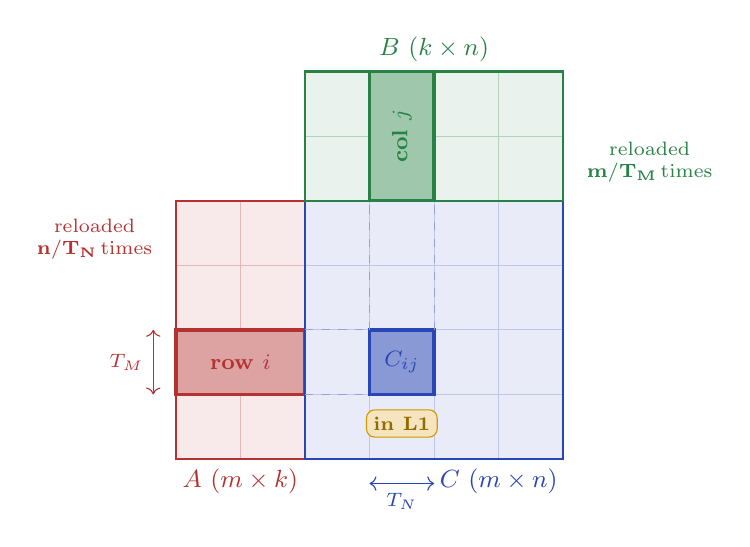
\begin{tikzpicture}[scale=0.82]
    %
    % Layout:   A (m×k) on the LEFT, B (k×n) on TOP, C (m×n) at the INTERSECTION.
    % This ensures the highlighted row-band of A and col-band of B
    % share the same y- and x-extents as the C tile.
    %
    % Coordinates (in units):
    %   A : x=[0,2],  y=[0,4]   (k=2 wide, m=4 tall)
    %   C : x=[2,6],  y=[0,4]   (n=4 wide, m=4 tall)
    %   B : x=[2,6],  y=[4,6]   (n=4 wide, k=2 tall)
    %
    % Tile chosen: row i (y=[1,2]) , col j (x=[3,4])  — each tile = 1×1 unit.

    %% ── A matrix (left) ──────────────────────────────────────────────
    \fill[matA!10] (0,0) rectangle (2,4);
    \draw[matA!35, thin] (0,0) grid[xstep=1, ystep=1] (2,4);
    \draw[matA, thick] (0,0) rectangle (2,4);
    % highlight row-band i (y=[1,2])
    \fill[matA!45] (0,1) rectangle (2,2);
    \draw[matA, very thick] (0,1) rectangle (2,2);
    \node[matA, font=\footnotesize\bfseries] at (1,1.5) {row $i$};
    % T_M brace
    \draw[matA, <->] (-0.35,1) -- node[left,font=\scriptsize]{$T_M$} (-0.35,2);
    % label + reload count
    \node[below, matA, font=\small] at (1,0) {$A$ ($m\times k$)};
    \node[matA, font=\scriptsize, align=center, left=5pt] at (0,3.4)
      {reloaded \\ $\mathbf{n/T_N}$\,times};

    %% ── C matrix (center) ───────────────────────────────────────────
    \fill[matC!10] (2,0) rectangle (6,4);
    \draw[matC!30, thin] (2,0) grid[xstep=1, ystep=1] (6,4);
    \draw[matC, thick] (2,0) rectangle (6,4);
    % highlight tile C_{ij} (x=[3,4], y=[1,2])
    \fill[matC!55] (3,1) rectangle (4,2);
    \draw[matC, very thick] (3,1) rectangle (4,2);
    \node[matC, font=\footnotesize\bfseries] at (3.5,1.5) {$C_{ij}$};
    % L1 badge
    \node[draw=cacheYellow, fill=cacheYellow!25, rounded corners=3pt,
          font=\scriptsize\bfseries, inner sep=2.5pt, text=cacheYellow!70!black]
      at (3.5, 0.55) {\raisebox{0pt}{in L1}};
    % T_N brace
    \draw[matC, <->] (3,-0.38) -- node[below,font=\scriptsize]{$T_N$} (4,-0.38);
    \node[below, matC, font=\small] at (5,0) {$C$ ($m\times n$)};
    % dashed alignment guides from tile to A and B
    \draw[matC!50, dashed, thin] (3,2) -- (3,4);   % left edge → B
    \draw[matC!50, dashed, thin] (4,2) -- (4,4);   % right edge → B
    \draw[matC!50, dashed, thin] (2,1) -- (3,1);   % bottom edge → A
    \draw[matC!50, dashed, thin] (2,2) -- (3,2);   % top edge → A

    %% ── B matrix (top) ──────────────────────────────────────────────
    \fill[matB!10] (2,4) rectangle (6,6);
    \draw[matB!35, thin] (2,4) grid[xstep=1, ystep=1] (6,6);
    \draw[matB, thick] (2,4) rectangle (6,6);
    % highlight col-band j (x=[3,4])
    \fill[matB!45] (3,4) rectangle (4,6);
    \draw[matB, very thick] (3,4) rectangle (4,6);
    \node[matB, font=\footnotesize\bfseries, rotate=90] at (3.5,5) {col $j$};
    % label + reload count
    \node[above, matB, font=\small] at (4,6) {$B$ ($k\times n$)};
    \node[matB, font=\scriptsize, align=center, right=5pt] at (6,4.6)
      {reloaded \\ $\mathbf{m/T_M}$\,times};

  \end{tikzpicture}
  \end{center}
\end{frame}

% ── Animation: C-stationary tiling step by step ──────────────────────────────
% Each overlay = one "click" in the presentation.
% Coordinate system (same as tiling slide):
%   A : x=[0,2],  y=[0,4]   (m=4 row-tiles × k=2 K-tiles)
%   C : x=[2,6],  y=[0,4]   (m=4 row-tiles × n=4 col-tiles)
%   B : x=[2,6],  y=[4,6]   (k=2 K-tiles   × n=4 col-tiles)
%   Tile chosen for animation: row i=0 (top, y=[3,4]), col j=0 (left, x=[2,3])
%   K-chunks: K0 = A col x=[0,1] / B row y=[5,6];  K1 = A col x=[1,2] / B row y=[4,5]
\begin{frame}<1-7>[t]{C-Stationary Tiling: Step by Step}

\vspace{-2pt}
\begin{center}
\begin{tikzpicture}[scale=0.77]

  % ── Step 1+: raw matrix outlines ──────────────────────────────────────────
  % A
  \fill[matA!12] (0,0) rectangle (2,4);
  \draw[matA, thick] (0,0) rectangle (2,4);
  \node[matA, font=\bfseries] at (1,2) {$A$};
  \node[below=1pt, matA, font=\scriptsize] at (1,0) {$m\times k$};
  % C
  \fill[matC!12] (2,0) rectangle (6,4);
  \draw[matC, thick] (2,0) rectangle (6,4);
  \node[matC, font=\bfseries] at (4,2) {$C$};
  \node[below=1pt, matC, font=\scriptsize] at (4,0) {$m\times n$};
  % B
  \fill[matB!12] (2,4) rectangle (6,6);
  \draw[matB, thick] (2,4) rectangle (6,6);
  \node[matB, font=\bfseries] at (4,5) {$B$};
  \node[above=1pt, matB, font=\scriptsize] at (4,6) {$k\times n$ (cheap)};

  % ── Step 2+: tile grid lines ───────────────────────────────────────────────
  \only<2->{
    \draw[matA!30, thin] (0,0) grid[xstep=1, ystep=1] (2,4);
    \draw[matC!25, thin] (2,0) grid[xstep=1, ystep=1] (6,4);
    \draw[matB!30, thin] (2,4) grid[xstep=1, ystep=1] (6,6);
    % T_M annotation (height of one row-tile, on left of A)
    \draw[<->, TechBlue!55, thin] (-0.45,3) -- node[left,font=\tiny]{$T_M$} (-0.45,4);
    % T_N annotation (width of one col-tile, below C)
    \draw[<->, TechBlue!55, thin] (2,-0.5) -- node[below,font=\tiny]{$T_N$} (3,-0.5);
    % T_K annotation (width of one K-tile, below A)
    \draw[<->, TechBlue!55, thin] (0,-0.5) -- node[below,font=\tiny]{$T_K$} (1,-0.5);
  }

  % ── Step 3+: outer-loop selection — C_{00}, A row 0, B col 0 ──────────────
  % A row-band 0 (persists from step 3 onward — same row for all j)
  \only<3->{
    \fill[matA!42] (0,3) rectangle (2,4);
    \draw[matA, very thick] (0,3) rectangle (2,4);
  }
  % B col-band 0 (steps 3–6 only; removed when j advances in step 7)
  \only<3-6>{
    \fill[matB!42] (2,4) rectangle (3,6);
    \draw[matB, very thick] (2,4) rectangle (3,6);
  }
  % C_{00} active tile (steps 3–6)
  \only<3-6>{
    \fill[matC!55] (2,3) rectangle (3,4);
    \draw[matC, very thick] (2,3) rectangle (3,4);
    \node[matC, font=\tiny\bfseries] at (2.5,3.5) {$C_{00}$};
    % dashed alignment guides
    \draw[gray!45, dashed, very thin] (3,4)--(3,3);
    \draw[gray!45, dashed, very thin] (2,4)--(2,3);
    \draw[gray!45, dashed, very thin] (0,3)--(2,3);
  }

  % ── Step 4–6: "in L1" badge on C tile ─────────────────────────────────────
  \only<4-6>{
    \node[draw=cacheYellow, fill=cacheYellow!22, rounded corners=2.5pt,
          font=\tiny\bfseries, inner sep=2pt, text=cacheYellow!70!black]
      at (2.5,2.62) {in L1};
    \draw[->, cacheYellow!70!black, very thin] (2.5,3.0) -- (2.5,2.8);
  }

  % ── Step 5: K-chunk 0 active in A and B ──────────────────────────────────
  % Drawn on top of the row/col-band fills — TikZ paints in order, so
  % the K-chunk highlight overwrites the lighter band fill where they overlap.
  \only<5>{
    % A: K-chunk 0 = left half of row 0 (x=[0,1], y=[3,4])
    \fill[matA!78] (0,3) rectangle (1,4);
    \draw[matA, very thick] (0,3) rectangle (1,4);
    \node[matA, font=\tiny] at (0.5,3.5) {$k_0$};
    % B: K-chunk 0 = top half of col 0 (x=[2,3], y=[5,6])
    \fill[matB!78] (2,5) rectangle (3,6);
    \draw[matB, very thick] (2,5) rectangle (3,6);
    \node[matB, font=\tiny, rotate=90] at (2.5,5.5) {$k_0$};
  }

  % ── Step 6: K-chunk 1 active, K-chunk 0 dimmed ───────────────────────────
  \only<6>{
    % A row 0: K0 dimmed, K1 active
    \fill[matA!18] (0,3) rectangle (1,4);   % dim K0
    \fill[matA!78] (1,3) rectangle (2,4);   % bright K1
    \draw[matA, very thick] (1,3) rectangle (2,4);
    \node[matA, font=\tiny] at (1.5,3.5) {$k_1$};
    % B col 0: K0 dimmed (y=[5,6]), K1 active (y=[4,5])
    \fill[matB!18] (2,5) rectangle (3,6);   % dim K0
    \fill[matB!78] (2,4) rectangle (3,5);   % bright K1
    \draw[matB, very thick] (2,4) rectangle (3,5);
    \node[matB, font=\tiny, rotate=90] at (2.5,4.5) {$k_1$};
  }

  % ── Step 7: C_{00} done; advance j → j+1 (B col 1, C_{01}) ───────────────
  \only<7>{
    % C_{00}: completed — dark fill, white "done" text
    \fill[matC!82] (2,3) rectangle (3,4);
    \draw[matC, very thick] (2,3) rectangle (3,4);
    \node[font=\tiny\bfseries, text=white] at (2.5,3.5) {done};
    % B col 1 selected (x=[3,4])
    \fill[matB!42] (3,4) rectangle (4,6);
    \draw[matB, very thick] (3,4) rectangle (4,6);
    % C_{01} active (x=[3,4], y=[3,4])
    \fill[matC!55] (3,3) rectangle (4,4);
    \draw[matC, very thick] (3,3) rectangle (4,4);
    \node[matC, font=\tiny\bfseries] at (3.5,3.5) {$C_{01}$};
    % alignment dashes for C_{01}
    \draw[gray!45, dashed, very thin] (4,4)--(4,3);
    \draw[gray!45, dashed, very thin] (3,4)--(3,3);
    % "in L1" on C_{01}
    \node[draw=cacheYellow, fill=cacheYellow!22, rounded corners=2.5pt,
          font=\tiny\bfseries, inner sep=2pt, text=cacheYellow!70!black]
      at (3.5,2.62) {in L1};
    \draw[->, cacheYellow!70!black, very thin] (3.5,3.0) -- (3.5,2.8);
  }

\end{tikzpicture}
\end{center}

\vspace{-4pt}
\begin{center}
\only<1>{\small Three matrices. $C = A \cdot B$.}
\only<2>{\small Partition into tiles of size $T_M \times T_N$ ($T_K$ in the K-dimension).}
\only<3>{\small Select $C_{00}$ — load corresponding $A$ row-band and $B$ col-band.}
\only<4>{\small $C_{00}$ enters L1 and \textbf{stays there} for all $K$ iterations.}
\only<5>{\small K-loop ($k=0$): \quad $C_{00} \mathrel{+}= A_{[i,k_0]} \times B_{[k_0,j]}$}
\only<6>{\small K-loop ($k=1$): \quad $C_{00} \mathrel{+}= A_{[i,k_1]} \times B_{[k_1,j]}$ \quad (only A/B K-chunks swap)}
\only<7>{\small $C_{00}$ complete. Advance $j$: \textbf{swap B col only} — A row-band stays $\Rightarrow$ compute $C_{01}$.}
\end{center}

\end{frame}

% ==============================================================================
\section{Theory}
% ==============================================================================

% ── T1: cost model ─────────────────────────────────────────────────────────────
\begin{frame}{The Memory Traffic Model}

  For one tile of $C$ (size $T_M \times T_N$, fast memory $M = T_M \cdot T_N$):

  \bigskip
  \begin{columns}[c]
    \begin{column}{0.54\textwidth}
      \renewcommand{\arraystretch}{1.6}
      \begin{tabular}{lll}
        \toprule
        Matrix & Reloads/elem & Cost \\
        \midrule
        $A$ (expensive) & $n / T_N$ & $\propto \dfrac{1}{T_N}$ \\[6pt]
        $B$ (cheap, $\rho$) & $m / T_M$ & $\propto \dfrac{\rho}{T_M}$ \\
        \bottomrule
      \end{tabular}

      \bigskip
      Minimize $\dfrac{1}{T_N} + \dfrac{\rho}{T_M}$ subject to $T_M \cdot T_N = M$.
    \end{column}

    \begin{column}{0.42\textwidth}
      \begin{block}{Optimal tile shape}
        \[
          \frac{T_N}{T_M} = \frac{1}{\rho}
        \]
        Wide tile when $B$ is cheap ($\rho < 1$).
      \end{block}

      \smallskip
      Examples:
      \begin{itemize}
        \item $\rho = 1$ (equal precision): $T_N = T_M$ \; \textbf{(square)}
        \item $\rho = 1/4$ (fp16 vs fp64): $T_N = 4\,T_M$
        \item $\rho \to 0$ (PRNG FIFO): widest feasible tile
      \end{itemize}
    \end{column}
  \end{columns}
\end{frame}

% ── T2: speedup formula ────────────────────────────────────────────────────────
\begin{frame}{Analytical Speedup over Square Tiles}

  \begin{columns}[c]
    \begin{column}{0.50\textwidth}
      At the optimal tile the two traffic terms balance:
      \[
        \underbrace{\frac{A\_PREC}{T_N}}_{\text{A traffic}} = \underbrace{\frac{B\_PREC}{T_M}}_{\text{B traffic}}
      \]
      Substituting $T_N^\star = \sqrt{M/\rho}$, $T_M^\star = \sqrt{M\rho}$:
      \[
        \mathrm{speedup} = \frac{\text{cost(square)}}{\text{cost(optimal)}}
                         = \frac{1 + \rho}{2\sqrt{\rho}}
      \]
    \end{column}

    \begin{column}{0.46\textwidth}
      \begin{block}{Predicted speedups}
        \renewcommand{\arraystretch}{1.35}
        \begin{tabular}{ccc}
          \toprule
          $\rho$ & $B$ precision & speedup \\
          \midrule
          $1$       & fp64 (8\,B) & $1.00\times$ \\
          $1/2$     & fp32 (4\,B) & $1.06\times$ \\
          $1/4$     & fp16 (2\,B) & $1.25\times$ \\
          $1/8$     & int8 (1\,B) & $1.59\times$ \\
          $\to 0$   & PRNG FIFO   & $\to \infty$ \\
          \bottomrule
        \end{tabular}
      \end{block}
      \smallskip
      {\footnotesize Speedup grows monotonically as $B$ becomes cheaper.}
    \end{column}
  \end{columns}
\end{frame}

% ── T3: wide-tile animation ────────────────────────────────────────────────────
% Same 7-step structure as the square-tile animation, but now T_M=1, T_N=4.
%
% Coordinate system (scale=0.70):
%   A : x=[0,2],  y=[0,4]    (m=4 row-tiles  ×  k=2 K-tiles)
%   C : x=[2,10], y=[0,4]    (m=4 row-tiles  ×  n=8 cols, T_N=4 → 2 wide col-tiles)
%   B : x=[2,10], y=[4,6]    (k=2 K-tiles    ×  n=8 cols, T_N=4 → 2 wide col-tiles)
%
%   Tile selected: row i=0 (top, y=[3,4])  col j=0 (left 4 cols, x=[2,6])
%   K-chunks: K0 = A col x=[0,1] / B row y=[5,6]
%             K1 = A col x=[1,2] / B row y=[4,5]
\begin{frame}<1-7>[t]{C-Stationary Tiling with Asymmetric Precision ($\rho=\tfrac{1}{4}$)}

\vspace{-2pt}
\begin{center}
\begin{tikzpicture}[scale=0.70]

  % ── Step 1+: raw matrix outlines ──────────────────────────────────────────
  % A  (tall and thin: m rows, only k=2 cols wide)
  \fill[matA!12] (0,0) rectangle (2,4);
  \draw[matA, thick] (0,0) rectangle (2,4);
  \node[matA, font=\bfseries] at (1,2) {$A$};
  \node[below=1pt, matA, font=\scriptsize] at (1,0) {$m\times k$};

  % C  (wide: m rows, n=8 cols)
  \fill[matC!12] (2,0) rectangle (10,4);
  \draw[matC, thick] (2,0) rectangle (10,4);
  \node[matC, font=\bfseries] at (6,2) {$C$};
  \node[below=1pt, matC, font=\scriptsize] at (6,0) {$m\times n$ (output)};

  % B  (wide and short: k=2 rows, n=8 cols)
  \fill[matB!12] (2,4) rectangle (10,6);
  \draw[matB, thick] (2,4) rectangle (10,6);
  \node[matB, font=\bfseries] at (6,5) {$B$};
  \node[above=1pt, matB, font=\scriptsize] at (6,6) {$k\times n$ \ (cheap, $\rho=\tfrac{1}{4}$)};

  % ── Step 2+: tile grid lines (T_M=1, T_N=4, T_K=1) ───────────────────────
  \only<2->{
    % A: K-cols every 1, rows every 1
    \draw[matA!30, thin] (0,0) grid[xstep=1, ystep=1] (2,4);
    % C: wide col-tiles every 4, rows every 1
    \draw[matC!25, thin] (2,0) grid[xstep=4, ystep=1] (10,4);
    % B: wide col-tiles every 4, K-rows every 1
    \draw[matB!30, thin] (2,4) grid[xstep=4, ystep=1] (10,6);
    % Dimension annotations
    \draw[<->, TechBlue!55, thin] (-0.45,3) -- node[left,font=\tiny]{$T_M{=}1$} (-0.45,4);
    \draw[<->, TechBlue!55, thin] (2,-0.5) -- node[below,font=\tiny]{$T_N{=}4$} (6,-0.5);
    \draw[<->, TechBlue!55, thin] (0,-0.5) -- node[below,font=\tiny]{$T_K$} (1,-0.5);
  }

  % ── Step 3+: select C_{00} (wide tile), A row 0, B col-band 0 ─────────────
  % A row 0 stays from step 3 onward (same row while advancing j)
  \only<3->{
    \fill[matA!42] (0,3) rectangle (2,4);
    \draw[matA, very thick] (0,3) rectangle (2,4);
  }
  % B col-band 0 (x=[2,6]) — steps 3-6 only
  \only<3-6>{
    \fill[matB!42] (2,4) rectangle (6,6);
    \draw[matB, very thick] (2,4) rectangle (6,6);
  }
  % C_{00} wide tile (x=[2,6], y=[3,4]) — steps 3-6
  \only<3-6>{
    \fill[matC!55] (2,3) rectangle (6,4);
    \draw[matC, very thick] (2,3) rectangle (6,4);
    \node[matC, font=\tiny\bfseries] at (4,3.5) {$C_{00}$};
    \draw[gray!45, dashed, very thin] (6,4)--(6,3);
    \draw[gray!45, dashed, very thin] (2,4)--(2,3);
    \draw[gray!45, dashed, very thin] (0,3)--(2,3);
  }

  % ── Step 4-6: "in L1" badge ────────────────────────────────────────────────
  \only<4-6>{
    \node[draw=cacheYellow, fill=cacheYellow!22, rounded corners=2.5pt,
          font=\tiny\bfseries, inner sep=2pt, text=cacheYellow!70!black]
      at (4,2.62) {in L1};
    \draw[->, cacheYellow!70!black, very thin] (4,3.0) -- (4,2.8);
  }

  % ── Step 5: K-chunk 0 ─────────────────────────────────────────────────────
  % A K0: x=[0,1], y=[3,4]    B K0: x=[2,6], y=[5,6]  (wide!)
  \only<5>{
    \fill[matA!78] (0,3) rectangle (1,4);
    \draw[matA, very thick] (0,3) rectangle (1,4);
    \node[matA, font=\tiny] at (0.5,3.5) {$k_0$};
    \fill[matB!78] (2,5) rectangle (6,6);
    \draw[matB, very thick] (2,5) rectangle (6,6);
    \node[matB, font=\tiny] at (4,5.5) {$k_0$};
  }

  % ── Step 6: K-chunk 1 (K0 dimmed) ─────────────────────────────────────────
  % A K1: x=[1,2], y=[3,4]    B K1: x=[2,6], y=[4,5]
  \only<6>{
    \fill[matA!18] (0,3) rectangle (1,4);
    \fill[matA!78] (1,3) rectangle (2,4);
    \draw[matA, very thick] (1,3) rectangle (2,4);
    \node[matA, font=\tiny] at (1.5,3.5) {$k_1$};
    \fill[matB!18] (2,5) rectangle (6,6);
    \fill[matB!78] (2,4) rectangle (6,5);
    \draw[matB, very thick] (2,4) rectangle (6,5);
    \node[matB, font=\tiny] at (4,4.5) {$k_1$};
  }

  % ── Step 7: C_{00} done; advance j → B col-band 1, C_{01} ─────────────────
  \only<7>{
    % C_{00} done
    \fill[matC!82] (2,3) rectangle (6,4);
    \draw[matC, very thick] (2,3) rectangle (6,4);
    \node[font=\tiny\bfseries, text=white] at (4,3.5) {done};
    % B col-band 1 (x=[6,10])
    \fill[matB!42] (6,4) rectangle (10,6);
    \draw[matB, very thick] (6,4) rectangle (10,6);
    % C_{01} wide tile
    \fill[matC!55] (6,3) rectangle (10,4);
    \draw[matC, very thick] (6,3) rectangle (10,4);
    \node[matC, font=\tiny\bfseries] at (8,3.5) {$C_{01}$};
    \draw[gray!45, dashed, very thin] (10,4)--(10,3);
    \draw[gray!45, dashed, very thin] (6,4)--(6,3);
    % "in L1" on C_{01}
    \node[draw=cacheYellow, fill=cacheYellow!22, rounded corners=2.5pt,
          font=\tiny\bfseries, inner sep=2pt, text=cacheYellow!70!black]
      at (8,2.62) {in L1};
    \draw[->, cacheYellow!70!black, very thin] (8,3.0) -- (8,2.8);
  }

\end{tikzpicture}
\end{center}

\vspace{-4pt}
\begin{center}
\only<1>{\small Wide matrices: $C$ has more columns than rows.}
\only<2>{\small Wide tile: $T_N = 4\,T_M$ — each C tile spans 4 columns, only 1 row.}
\only<3>{\small Select $C_{00}$ (wide) — A row-band is \textbf{thin}; B col-band is \textbf{wide}.}
\only<4>{\small $C_{00}$ enters L1 and stays. The wide C tile fits because $T_M$ is small.}
\only<5>{\small K-loop ($k=0$): \quad $C_{00} \mathrel{+}= A_{[i,k_0]} \times B_{[k_0,\,j:j+4]}$}
\only<6>{\small K-loop ($k=1$): \quad $C_{00} \mathrel{+}= A_{[i,k_1]} \times B_{[k_1,\,j:j+4]}$}
\only<7>{\small $C_{00}$ done. Swap $B$ col-band (2 total). $A$ row stays.
         \quad $A$ reloads: $n/T_N = \mathbf{2}$. \quad $B$ reloads: $m/T_M = \mathbf{4}$ (cheap — OK!)}
\end{center}

\end{frame}

% ── bridge ─────────────────────────────────────────────────────────────────────
% ── Slide 5: the question ──────────────────────────────────────────────────────
\begin{frame}{The Central Question}

  \begin{columns}[c]
    \begin{column}{0.5\textwidth}
      \textbf{Theory says:} reshape the tile — wide beats square when $\rho < 1$.

      \bigskip
      \begin{center}
      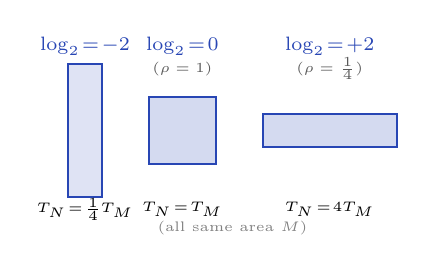
\begin{tikzpicture}[scale=0.60]
        % Three tiles with identical area ≈ 2 sq.\ units,
        % accurate TN/TM ratios: 1/4 : 1 : 4.
        % Gaps widened to 1.0 unit so log₂ labels don't overlap.
        % All log₂ labels pinned to y=3.2; ratio labels to y=-0.25.
        %   Tall:   x=[0,    0.71],  center=0.355
        %   Square: x=[1.71, 3.12],  center=2.415
        %   Wide:   x=[4.12, 6.95],  center=5.535

        % ── Tall tile (log₂ = -2, TN/TM = 1/4) ─────────────────────────
        \fill[matC!15] (0, 0) rectangle (0.71, 2.83);
        \draw[matC, thick] (0, 0) rectangle (0.71, 2.83);
        \node[font=\scriptsize\bfseries, matC] at (0.355, 3.2)
              {$\log_2\!=\!{-2}$};
        \node[font=\tiny] at (0.355, -0.25) {$T_N\!=\!\tfrac{1}{4}T_M$};

        % ── Square tile (log₂ = 0, TN/TM = 1) ──────────────────────────
        \fill[matC!20] (1.71, 0.71) rectangle (3.12, 2.12);
        \draw[matC, thick] (1.71, 0.71) rectangle (3.12, 2.12);
        \node[font=\scriptsize\bfseries, matC] at (2.415, 3.2)
              {$\log_2\!=\!0$};
        \node[font=\tiny, gray!70!black] at (2.415, 2.72) {($\rho=1$)};
        \node[font=\tiny] at (2.415, -0.25) {$T_N\!=\!T_M$};

        % ── Wide tile (log₂ = +2, TN/TM = 4) ───────────────────────────
        \fill[matC!20] (4.12, 1.06) rectangle (6.95, 1.77);
        \draw[matC, thick] (4.12, 1.06) rectangle (6.95, 1.77);
        \node[font=\scriptsize\bfseries, matC] at (5.535, 3.2)
              {$\log_2\!=\!{+2}$};
        \node[font=\tiny, gray!70!black] at (5.535, 2.72)
              {($\rho=\tfrac{1}{4}$)};
        \node[font=\tiny] at (5.535, -0.25) {$T_N\!=\!4T_M$};

        % ── Same-area note ───────────────────────────────────────────────
        \node[font=\tiny, gray] at (3.475, -0.65) {(all same area $M$)};
      \end{tikzpicture}
      \end{center}
    \end{column}

    \begin{column}{0.46\textwidth}
      \textbf{But does it hold in practice?}

      \begin{itemize}
        \item Real caches have finite size, eviction policies, set conflicts
        \item $C$ tile must fit in L1 — limits how wide we can go
        \item PRNG FIFO changes the bandwidth model entirely
      \end{itemize}

      \bigskip
      \begin{block}{Our approach}
        Build a \textbf{cycle-accurate cache simulator} and validate (or refute)
        the theory across a wide sweep of tile shapes, cache sizes, and
        precision ratios.
      \end{block}
    \end{column}
  \end{columns}
\end{frame}

% ==============================================================================
\section{The Simulator}
% ==============================================================================

% ── UML: architecture ─────────────────────────────────────────────────────────
\begin{frame}{Simulator Architecture}
  \vspace{-0.15cm}
  \centering
  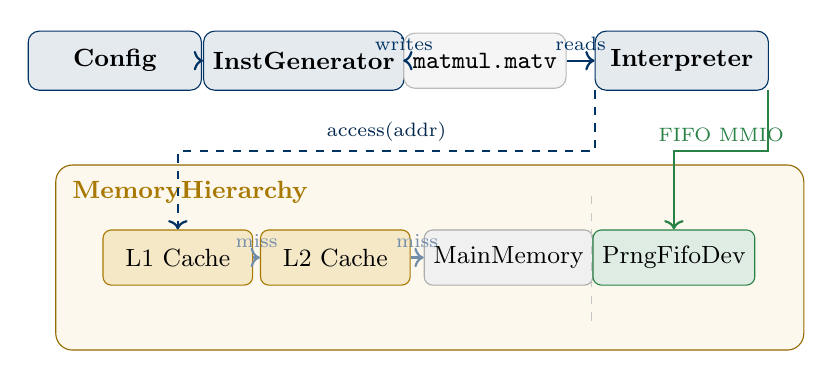
\begin{tikzpicture}[
    % scale=1: every TikZ unit = 1 cm, minimum width/height in cm are consistent
    comp/.style={draw=TechBlue, fill=TechBlue!10, rounded corners=4pt,
                 minimum width=2.2cm, minimum height=0.75cm,
                 align=center, font=\small\bfseries},
    cache/.style={draw=cacheYellow!80!black, fill=cacheYellow!22,
                  rounded corners=3pt, minimum width=1.9cm, minimum height=0.7cm,
                  align=center, font=\small},
    fifos/.style={draw=matB, fill=matB!15, rounded corners=3pt,
                  minimum width=1.9cm, minimum height=0.7cm,
                  align=center, font=\small},
    mems/.style={draw=gray!65, fill=gray!12, rounded corners=3pt,
                 minimum width=1.9cm, minimum height=0.7cm,
                 align=center, font=\small},
    filebox/.style={draw=gray!55, fill=gray!8, rounded corners=4pt,
                    minimum width=2.0cm, minimum height=0.7cm,
                    align=center, font=\small\ttfamily},
    arr/.style={->, thick, TechBlue},
    miss/.style={->, thick, TechBlue!55}
  ]

  % ── Top row: instruction-generation pipeline (left to right) ─────────────
  \node[comp]    (cfg)    at (-4.2, 2.0) {Config};
  \node[comp]    (gen)    at (-1.8, 2.0) {InstGenerator};
  \node[filebox] (matv)   at ( 0.5, 2.0) {matmul.matv};
  \node[comp]    (interp) at ( 3.0, 2.0) {Interpreter};

  \draw[arr] (cfg)  -- (gen);
  \draw[arr] (gen)  -- node[above, font=\scriptsize]{writes} (matv);
  \draw[arr] (matv) -- node[above, font=\scriptsize]{reads}  (interp);

  % ── MemoryHierarchy subsystem box ─────────────────────────────────────────
  \node[draw=cacheYellow!70!black, fill=cacheYellow!7, rounded corners=6pt,
        minimum width=9.5cm, minimum height=2.35cm]
        (mhbox) at (-0.2, -0.5) {};
  \node[font=\small\bfseries, text=cacheYellow!80!black,
        anchor=north west, inner sep=6pt] at (mhbox.north west)
        {MemoryHierarchy};

  % Four internal components (evenly spaced, all on the same row)
  \node[cache] (l1)   at (-3.4, -0.5) {L1 Cache};
  \node[cache] (l2)   at (-1.4, -0.5) {L2 Cache};
  \node[mems]  (dram) at ( 0.8, -0.5) {MainMemory};
  \node[fifos] (fifo) at ( 2.9, -0.5) {PrngFifoDev};

  \draw[miss] (l1)   -- node[above, font=\scriptsize]{miss} (l2);
  \draw[miss] (l2)   -- node[above, font=\scriptsize]{miss} (dram);

  % Dashed divider: cache chain vs FIFO bypass
  \draw[gray!45, dashed, thin] (1.85, -1.3) -- (1.85, 0.35);

  % ── Connections from Interpreter ─────────────────────────────────────────
  % access(addr): L-shaped path down then left to L1
  %   interp.south west ≈ (1.9, 1.625) → down to y=0.85 → left to l1.north x
  \draw[arr, dashed]
        (1.9, 1.625)
        -- (1.9, 0.85)
        -- (-3.4, 0.85)
        -- (l1.north);
  \node[font=\scriptsize, TechBlue!75!black, above] at (-0.75, 0.85)
        {access(addr)};

  % FIFO MMIO: L-shaped path down then left to PrngFifoDev
  %   interp.south east ≈ (4.1, 1.625) → down to y=0.85 → left to fifo.north x
  \draw[->, thick, matB]
        (4.1, 1.625)
        -- (4.1, 0.85)
        -- (2.9, 0.85)
        -- (fifo.north);
  \node[font=\scriptsize, matB, above] at (3.5, 0.85) {FIFO MMIO};

  \end{tikzpicture}
\end{frame}

% ── S1: overview ───────────────────────────────────────────────────────────────
\begin{frame}{Simulator Overview}

  \begin{columns}[c]

    % Left: pipeline diagram
    \begin{column}{0.52\textwidth}
      \centering
      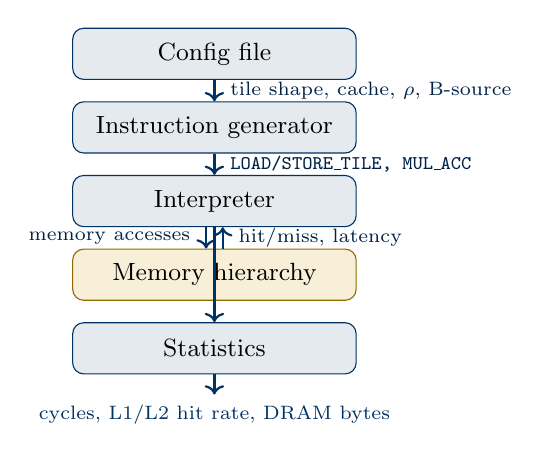
\begin{tikzpicture}[scale=0.85,
          box/.style={draw=TechBlue, fill=TechBlue!10, rounded corners=4pt,
                      minimum width=3.6cm, minimum height=0.65cm,
                      align=center, font=\small},
          arr/.style={->, TechBlue, thick},
          lbl/.style={font=\scriptsize, text=TechBlue!70!black, align=left}
        ]
        \node[box] (cfg)    at (0, 0)    {Config file};
        \node[box] (gen)    at (0,-1.1)  {Instruction generator};
        \node[box] (interp) at (0,-2.2)  {Interpreter};
        \node[box, fill=cacheYellow!15, draw=cacheYellow!70!black]
                   (mem)    at (0,-3.3)  {Memory hierarchy};
        \node[box] (stat)   at (0,-4.4)  {Statistics};

        \draw[arr] (cfg)    -- node[lbl, right=2pt]{tile shape, cache, $\rho$, B-source} (gen);
        \draw[arr] (gen)    -- node[lbl, right=2pt]{\texttt{LOAD/STORE\_TILE, MUL\_ACC}} (interp);
        % Bidirectional interp <-> mem: offset left/right to avoid overlap
        \draw[arr, transform canvas={xshift=-3pt}]
              (interp.south) -- node[lbl, left=2pt]{memory accesses} (mem.north);
        \draw[arr, transform canvas={xshift=3pt}]
              (mem.north) -- node[lbl, right=2pt]{hit/miss, latency} (interp.south);
        \draw[arr] (interp) -- node[lbl, right=2pt]{} (stat);
        \draw[arr] (stat.south) -- ++(0,-0.3)
              node[below, font=\scriptsize]{cycles, L1/L2 hit rate, DRAM bytes};
      \end{tikzpicture}
    \end{column}

    % Right: key facts
    \begin{column}{0.44\textwidth}
      \begin{block}{What it is}
        Cycle-accurate C++ simulator for tiled $C{=}A{\cdot}B$ with
        configurable cache hierarchy and B-source.
      \end{block}

      \smallskip
      \textbf{3 instruction types:}\\[2pt]
      \texttt{LOAD\_TILE} \quad \texttt{STORE\_TILE} \quad \texttt{TILE\_MUL\_ACC}

      \smallskip
      \textbf{Key config knobs:}
      \begin{itemize}\setlength\itemsep{1pt}
        \item Matrix dims and precision ratio $\rho$
        \item Tile shape ($T_M, T_N, T_K$)
        \item L1/L2: size, line size, associativity
        \item B-source: \texttt{mem} / \texttt{prng\_fifo}
        \item Loop ordering: C-stat.\ / B-stat.
      \end{itemize}
    \end{column}

  \end{columns}
\end{frame}

% ── S2: memory hierarchy ───────────────────────────────────────────────────────
\begin{frame}{Memory Hierarchy and B-Source Modes}

  \begin{columns}[T]

    % Left column: mem mode diagram
    \begin{column}{0.46\textwidth}
      \textbf{Mode: \texttt{mem}} \quad (B stored in DRAM)

      \smallskip
      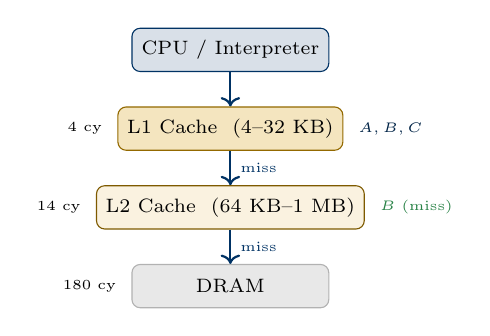
\begin{tikzpicture}[
          box/.style={draw, rounded corners=3pt, minimum width=2.5cm,
                      minimum height=0.55cm, align=center, font=\scriptsize},
          arr/.style={->, thick}
        ]
        \node[box, fill=TechBlue!15, draw=TechBlue] (cpu) at (0,0) {CPU / Interpreter};
        \node[box, fill=cacheYellow!25, draw=cacheYellow!70!black]
              (l1)  at (0,-1.0) {L1 Cache \ (4--32 KB)};
        \node[box, fill=cacheYellow!12, draw=cacheYellow!60!black]
              (l2)  at (0,-2.0) {L2 Cache \ (64 KB--1 MB)};
        \node[box, fill=gray!18, draw=gray!60]
              (dram)at (0,-3.0) {DRAM};

        \draw[arr, TechBlue]  (cpu)  -- (l1);
        \draw[arr, TechBlue]  (l1)   -- node[right,font=\tiny]{miss} (l2);
        \draw[arr, TechBlue]  (l2)   -- node[right,font=\tiny]{miss} (dram);

        \node[font=\tiny, left=2pt] at (l1.west)   {4 cy};
        \node[font=\tiny, left=2pt] at (l2.west)   {14 cy};
        \node[font=\tiny, left=2pt] at (dram.west) {180 cy};

        \node[font=\tiny, right=2pt, text=TechBlue!70!black] at (l1.east)  {$A, B, C$};
        \node[font=\tiny, right=2pt, matB]                   at (l2.east)  {$B$ (miss)};
      \end{tikzpicture}

      \smallskip
      All matrices compete for L1 space.\\
      B tile evicts A or C lines if L1 is full.
    \end{column}

    % Right column: prng_fifo mode
    \begin{column}{0.50\textwidth}
      \textbf{Mode: \texttt{prng\_fifo}} \quad (B from hardware FIFO)

      \smallskip
      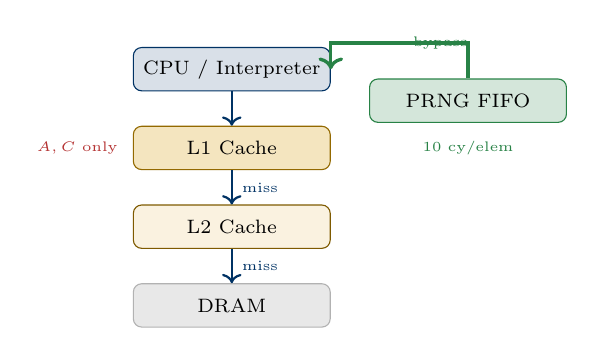
\begin{tikzpicture}[
          box/.style={draw, rounded corners=3pt, minimum width=2.5cm,
                      minimum height=0.55cm, align=center, font=\scriptsize},
          arr/.style={->, thick}
        ]
        \node[box, fill=TechBlue!15, draw=TechBlue] (cpu)  at (0,0) {CPU / Interpreter};
        \node[box, fill=cacheYellow!25, draw=cacheYellow!70!black]
              (l1)   at (0,-1.0) {L1 Cache};
        \node[box, fill=cacheYellow!12, draw=cacheYellow!60!black]
              (l2)   at (0,-2.0) {L2 Cache};
        \node[box, fill=gray!18, draw=gray!60]
              (dram) at (0,-3.0) {DRAM};
        \node[box, fill=matB!20, draw=matB]
              (fifo) at (3.0,-0.4) {PRNG FIFO};

        \draw[arr, TechBlue]  (cpu)  -- (l1);
        \draw[arr, TechBlue]  (l1)   -- node[right,font=\tiny]{miss} (l2);
        \draw[arr, TechBlue]  (l2)   -- node[right,font=\tiny]{miss} (dram);
        % FIFO bypasses L1 entirely — routed around the right side
        \draw[arr, matB, very thick]
              (fifo.north) -- ++(0, 0.45) -|
              node[near start, right=1pt, font=\tiny, matB]{bypass} (cpu.east);

        \node[matA, font=\tiny, left=2pt] at (l1.west)   {$A, C$ only};
        \node[matB, font=\tiny, below=3pt] at (fifo.south) {10 cy/elem};
      \end{tikzpicture}

      \smallskip
      B generated at fixed cost per element.\\
      \textbf{No cache pressure from B} — L1 fully available for $A$ and $C$.\\
      Models extreme case $\rho \to 0$.
    \end{column}

  \end{columns}

  \medskip
  \begin{center}
    \small Replacement policies: \textbf{LRU} (default) $\cdot$ FIFO $\cdot$ MRU $\cdot$ Random
  \end{center}
\end{frame}

% ── S3: loop orderings ─────────────────────────────────────────────────────────
\begin{frame}{Loop Orderings: C-Stationary vs B-Stationary}

  \begin{columns}[T]

    \begin{column}{0.47\textwidth}
      \textbf{C-stationary}
      \begin{block}{}
        \ttfamily\footnotesize
        \textbf{for} i (row-tiles of C):\\
        \quad \textbf{for} j (col-tiles of C):\\
        \quad\quad C[i,j] $\to$ L1 \textcolor{cacheYellow!70!black}{(stays all K)}\\
        \quad\quad \textbf{for} k:\\
        \quad\quad\quad load A[i,k]\\
        \quad\quad\quad load B[k,j]\\
        \quad\quad\quad C[i,j] += A*B\\
        \quad\quad write C[i,j]
      \end{block}
      \smallskip
      \begin{itemize}
        \item $C$ tile resident in L1 across all $K$
        \item $A$: reloaded $n/T_N$ times per element
        \item $B$: reloaded $m/T_M$ times per element
        \item \textbf{Best when $C$ tile fits in L1}
      \end{itemize}
    \end{column}

    \begin{column}{0.47\textwidth}
      \textbf{B-stationary}
      \begin{block}{}
        \ttfamily\footnotesize
        \textbf{for} j (col-tiles of B):\\
        \quad \textbf{for} k (row-tiles of B):\\
        \quad\quad B[k,j] $\to$ L1 \textcolor{matB}{(stays all M)}\\
        \quad\quad \textbf{for} i:\\
        \quad\quad\quad load A[i,k]\\
        \quad\quad\quad load C[i,j]\\
        \quad\quad\quad C[i,j] += A*B\\
        \quad\quad\quad store C[i,j]
      \end{block}
      \smallskip
      \begin{itemize}
        \item $B$ tile resident in L1 across all $M$
        \item $C$: reloaded $k/T_K$ times per element
        \item $A$: reloaded $n/T_N$ times per element
        \item \textbf{Better when B is expensive (large $\rho$)}
      \end{itemize}
    \end{column}

  \end{columns}
\end{frame}

% ── S4: experiment setup ───────────────────────────────────────────────────────
\begin{frame}{Experiment Setup}

  \begin{columns}[T]

    \begin{column}{0.48\textwidth}
      \textbf{Fixed workload}
      \begin{itemize}
        \item Square matrix: $m = n = k = 96$
        \item A precision: 8 B/elem (fp64)
        \item B precision: $\rho \in \{1, \tfrac{1}{2}, \tfrac{1}{4}\}$
      \end{itemize}

      \bigskip
      \textbf{Swept: tile shapes}
      \begin{itemize}
        \item $T_M, T_N \in \{4, 8, 12, 16, 24, 32, 48, 96\}$
        \item $T_K \in \{8, 16, 24, 32, 48, 96\}$
        \item 343 tile shape combinations per config
      \end{itemize}
    \end{column}

    \begin{column}{0.48\textwidth}
      \textbf{Swept: hardware parameters}
      \renewcommand{\arraystretch}{1.25}
      \begin{tabular}{ll}
        \toprule
        Parameter & Values \\
        \midrule
        L1 size     & 4, 8, 16, 32 KB \\
        Line size   & 16, 32, 64 B \\
        Associativity & 1, 2, 4, 8, 16-way \\
        \midrule
        B-source    & \texttt{mem}, \texttt{prng\_fifo} \\
        Stationary  & C, B \\
        Repl.\ policy & LRU, FIFO, MRU, Random \\
        \bottomrule
      \end{tabular}

      \bigskip
      \textbf{$\approx\!20{,}000$ simulator runs}\\
      {\footnotesize Results cached; full sweep $\sim$minutes on a laptop.}
    \end{column}

  \end{columns}
\end{frame}

% ==============================================================================
\section{Results}
% ==============================================================================

% ── R1a: Tile shape sweep — Setup & Hypothesis ────────────────────────────────
\begin{frame}{Exp.\ 1 — Does $\rho$ Drive the Optimal Tile Shape?}
  \framesubtitle{Setup \& Hypothesis}

  \begin{columns}[T]

    \begin{column}{0.47\textwidth}
      \textbf{What we test}\\[4pt]
      Sweep all 343 valid tile shapes $(T_M, T_N, T_K)$ on a $96^3$ matmul
      and record total simulated cycles for each $\rho$ regime.

      \medskip
      \textbf{Setup}
      \begin{itemize}\setlength\itemsep{2pt}
        \item Matrix dimensions: $m=n=k=96$
        \item Ordering: C-stationary
        \item 16\,KB L1, 64\,B lines, LRU policy
        \item B-source: memory \textbf{and} PRNG FIFO
      \end{itemize}
    \end{column}

    \begin{column}{0.49\textwidth}
      \textbf{Hypothesis}\\[4pt]
      The single-level L1 model predicts the DRAM-optimal tile satisfies:
      \[
        \frac{T_N}{T_M} = \frac{1}{\rho}
      \]
      Intuition: A (fp64) reloads cost $1/\rho{\times}$ more than B reloads.
      Using a larger $T_N$ and smaller $T_M$ balances DRAM traffic.

      \smallskip
      \begin{itemize}\setlength\itemsep{2pt}
        \item $\rho=1$: square tile ($T_N=T_M$)
        \item $\rho=\tfrac{1}{4}$: 4:1 wide tile
        \item PRNG FIFO: $\rho_\text{eff}\!\to0 \Rightarrow$ widest tile wins
      \end{itemize}
    \end{column}

  \end{columns}
\end{frame}

% ── R1b: Tile shape sweep — Results (graph) ───────────────────────────────────
\begin{frame}{Exp.\ 1 — Does $\rho$ Drive the Optimal Tile Shape?}
  \framesubtitle{Results}

  \vspace{0.05cm}
  \centering
  \includegraphics[width=\textwidth, trim=0 0 0 4pt, clip]{exp1_tile_shape}

  \vspace{0.1cm}
  \small
  Each panel: cycles vs.\ tile aspect ratio $\log_2(T_N/T_M)$.\\
  Solid line = best-per-ratio envelope.
  Filled dot = empirical minimum.
  Dashed line = theory prediction.
\end{frame}

% ── R1c: Tile shape sweep — Findings table ────────────────────────────────────
\begin{frame}{Exp.\ 1 — Does $\rho$ Drive the Optimal Tile Shape?}
  \framesubtitle{Detailed Findings}

  \begin{columns}[T]

    \begin{column}{0.38\textwidth}
      \textbf{Key observations}
      \begin{itemize}\setlength\itemsep{1pt}
        \item $\rho=1$, $\rho=1/4$: theory exactly matched
        \item FIFO: max-wide tile wins (B has zero cache footprint)
        \item $\rho=1/2$ anomaly: empirical optimum is \emph{opposite} to theory
      \end{itemize}

      \smallskip
      \textbf{Anomaly:} $T_M{=}96$ spans the full M dimension — A persists in L2 across
      $j$-iterations (two-level effect, outside the model).
    \end{column}

    \begin{column}{0.58\textwidth}
      \textbf{Best tile per regime} (min cycles)
      \renewcommand{\arraystretch}{1.3}
      \small
      \begin{tabular}{llccc}
        \toprule
        $\rho$ & B-source & Best $T_M{\times}T_N$ & $T_N/T_M$ & Theory \\
        \midrule
        $1$   & mem (fp64) & $32{\times}32$ & $1.0$ & $1.0$ \\
        $1/4$ & mem (asym) & $24{\times}96$ & $4.0$ & $4.0$ \\
        $1$   & mem (fp32) & $96{\times}32$ & $0.3$ & $1.0$ \\[2pt]
        $1$   & FIFO       & $32{\times}96$ & $3.0$ & ${\to}\infty$ \\
        $1/4$ & FIFO       & $32{\times}96$ & $3.0$ & ${\to}\infty$ \\
        \bottomrule
      \end{tabular}
    \end{column}

  \end{columns}
\end{frame}

% ── R1d: Tile shape sweep — Verdict ───────────────────────────────────────────
\begin{frame}{Exp.\ 1 — Verdict}

  \begin{columns}[T]

    \begin{column}{0.48\textwidth}
      \textcolor{matB!80!black}{\large\bfseries Partial match}\\[6pt]
      Theory correctly predicts the direction for:
      \begin{itemize}\setlength\itemsep{5pt}
        \item[\textcolor{matB!80!black}{\checkmark}]
          $\rho=1$: square tile — \textit{exactly matched}
        \item[\textcolor{matB!80!black}{\checkmark}]
          $\rho=1/4$: 4:1 wide tile — \textit{exactly matched}
        \item[\textcolor{matB!80!black}{\checkmark}]
          PRNG FIFO: maximally wide — \textit{confirms $\rho_\text{eff}\to0$}
      \end{itemize}
    \end{column}

    \begin{column}{0.48\textwidth}
      \textcolor{matA}{\large\bfseries Anomaly: Sym.\ Single (fp32)}\\[4pt]
      Empirical best: $96{\times}32$, $T_N/T_M\approx0.3$\\
      Theory predicts: $T_N/T_M=1.0$ (square tile, since $\rho=1$)

      \medskip
      \textbf{Root cause:} $T_M=96$ spans the full M dimension.
      Smaller elements (4\,B vs.\ 8\,B) let the entire A tile persist in L2
      across all $j$-iterations — a two-level caching effect the single-level model ignores.

      \medskip
      \begin{block}{\small Takeaway}
        \small
        The model is a good first approximation but needs
        extension for multi-level cache effects.
      \end{block}
    \end{column}

  \end{columns}
\end{frame}

% ── R1e: Anomaly — L2 Buffering Hypothesis ────────────────────────────────────
\begin{frame}{Exp.\ 1 — Anomaly: L2 Buffering Hypothesis}
  \framesubtitle{Why does $96{\times}32{\times}96$ win for Sym.\ Single?}

  \begin{columns}[T]

    \begin{column}{0.50\textwidth}
      \textcolor{matA}{\bfseries Observation}\\[3pt]
      Empirical best is $96{\times}32{\times}96$ (tall tile, $T_N/T_M \approx 0.3$);
      theory predicts the \emph{square} tile ($T_N/T_M = 1$, since $\rho=1$).

      \smallskip
      \textbf{Proposed mechanism:} $T_M = 96 = M$, so only \textbf{one A-strip} exists
      in C-stationary order. The same A-tile feeds all $N/T_N = 3$~$j$-iterations.

      \smallskip
      A-tile size: $96 \times 96 \times 4\,\text{B} = \mathbf{36\,\text{KB}}$\\
      Default L2: $64\,\text{KB} > 36\,\text{KB}$
      $\Rightarrow$ A is loaded once and \emph{buffered} in L2.

      \smallskip
      The single-level model ignores this: it assumes every A access goes to DRAM.
    \end{column}

    \begin{column}{0.46\textwidth}
      \textcolor{TechBlue}{\bfseries Experiment}\\[3pt]
      Re-run the full 343-shape sweep (Sym.\ Single, C-stationary, mem)
      under two L2 sizes:

      \smallskip
      \begin{tabular}{lcc}
        \hline
        Condition & L2 & A-tile fits? \\
        \hline
        Default & 64\,KB & \textcolor{matB!80!black}{\checkmark} yes \\
        Tiny    &  8\,KB & $\times$\ no \\
        \hline
      \end{tabular}

      \smallskip
      \textbf{Prediction:} with L2\,=\,8\,KB $<$ 36\,KB the anomalous tile
      loses its advantage; the optimal tile shifts toward the theory-predicted
      square.
    \end{column}

  \end{columns}
\end{frame}

% ── R1f: Anomaly — Confirmed ──────────────────────────────────────────────────
\begin{frame}{Exp.\ 1 — Anomaly: Confirmed}

  \begin{columns}[T]

    \begin{column}{0.55\textwidth}
      \includegraphics[width=\textwidth]{exp1_l2_anomaly}
    \end{column}

    \begin{column}{0.43\textwidth}
      \small
      \textbf{Rank reversal:}

      \smallskip
      {\scriptsize
      \begin{tabular}{lcc}
        \hline
        Tile & 64\,KB & 8\,KB \\
        \hline
        $96\times32\times96$ & \#1\,(2.70M) & \#26\,(3.76M) \\
        $32\times32\times96$ & \#21\,(2.86M) & \#70\,(4.00M) \\
        $32\times32\times24$ & \#96\,(3.03M) & \#3\,(3.50M) \\
        \hline
      \end{tabular}
      }

      \smallskip
      With large L2 the anomalous tile exploits cached A
      reuse. With tiny L2 it falls from \#1 to \#26, while
      the square tile $32{\times}32{\times}24$ jumps from
      \#96 to \#3 — exactly as predicted.

      \smallskip
      \begin{block}{\small Conclusion}
        \small
        The anomaly is a \textbf{multi-level caching} effect:
        A fits in L2 and is reused across $j$-iterations —
        invisible to the single-level model.
      \end{block}
    \end{column}

  \end{columns}
\end{frame}

% ── R2a: H1 unconstrained — Setup & Hypothesis ────────────────────────────────
\begin{frame}{Exp.\ 2 — Unconstrained Optimal Aspect Ratio (Hypothesis 1)}
  \framesubtitle{Setup \& Hypothesis}

  \begin{columns}[T]

    \begin{column}{0.47\textwidth}
      \textbf{What we test}\\[4pt]
      Run the tile sweep with a very large L1 (256\,KB) so the full working set
      fits in cache, eliminating the capacity constraint.
      We measure DRAM bytes as a function of tile aspect ratio.

      \medskip
      \textbf{Setup}
      \begin{itemize}\setlength\itemsep{2pt}
        \item Matrix: $512^3$, C-stationary
        \item L1: 256\,KB (fits whole working set)
        \item 49 tile shapes across $\log_2(T_N/T_M) \in [-6, +6]$
        \item B-source: memory
      \end{itemize}
    \end{column}

    \begin{column}{0.49\textwidth}
      \textbf{Hypothesis 1}\\[3pt]
      Extending the tiling analysis of Lam et al.\ (1991) to mixed precision:
      when L1 is large enough that no matrix is evicted, the DRAM-minimising
      tile satisfies $T_N^*/T_M^* = 1/\rho$, with DRAM reduction
      $1 - 2\sqrt{\rho}/(1{+}\rho)$ vs a square tile.

      \smallskip
      \begin{tabular}{ccc}
        \hline
        $\rho$ & Opt.\ $\log_2$ & DRAM reduction \\
        \hline
        $1$     & $0$  & $0\%$ \\
        $1/2$   & $+1$ & $5.7\%$ \\
        $1/4$   & $+2$ & $20\%$ \\
        $1/8$   & $+3$ & $37\%$ \\
        \hline
      \end{tabular}
    \end{column}

  \end{columns}
\end{frame}

% ── R2b: H1 unconstrained — Results (graph) ───────────────────────────────────
\begin{frame}{Exp.\ 2 — Unconstrained Optimal Aspect Ratio (Hypothesis 1)}
  \framesubtitle{Results}

  \centering
  \includegraphics[width=\textwidth, trim=0 0 0 4pt, clip]{exp2_h1_unconstrained}

  \vspace{0.05cm}
  {\small DRAM normalised to square tile. \ Dashed = theory. \ Filled dot = empirical min.}
\end{frame}

% ── R2c: H1 unconstrained — Detailed findings ─────────────────────────────────
\begin{frame}{Exp.\ 2 — Unconstrained Optimal Aspect Ratio (Hypothesis 1)}
  \framesubtitle{Detailed Findings}

  \begin{columns}[T]

    \begin{column}{0.42\textwidth}
      \textbf{Key observations}
      \begin{itemize}\setlength\itemsep{3pt}
        \item Empirical minima are on the \emph{tall} side ($\log_2 < 0$) — opposite to theory
        \item The DRAM landscape is nearly flat: best tile is only $1$–$3\%$ better than square
        \item $\rho=1/8$: curve is completely flat — B is so cheap it barely contributes to DRAM
        \item Theory predicts up to $37\%$ gain; measured gain $\le 2.4\%$
      \end{itemize}
    \end{column}

    \begin{column}{0.54\textwidth}
      \renewcommand{\arraystretch}{1.1}
      \small
      \begin{tabular}{ccccc}
        \toprule
        & \multicolumn{2}{c}{$\log_2(T_N/T_M)$} & \multicolumn{2}{c}{DRAM vs.\ square} \\
        \cmidrule(lr){2-3}\cmidrule(lr){4-5}
        $\rho$ & Theory & Empirical & Theory & Measured \\
        \midrule
        $1$     & $\phantom{+}0$  & $\phantom{+}0$  & $1.000$ & $1.000$ \\
        $1/2$   & $+1$ & $-2$ & $0.943$ & $0.987$ \\
        $1/4$   & $+2$ & $-1$ & $0.800$ & $0.976$ \\
        $1/8$   & $+3$ & $\phantom{+}0$  & $0.629$ & $1.000$ \\
        \bottomrule
      \end{tabular}
    \end{column}

  \end{columns}
\end{frame}

% ── R2d: H1 unconstrained — Verdict ───────────────────────────────────────────
\begin{frame}{Exp.\ 2 — Verdict}

  \begin{columns}[T]

    \begin{column}{0.48\textwidth}
      \textcolor{matA}{\large\bfseries Diverges from theory}\\[6pt]
      \begin{itemize}\setlength\itemsep{5pt}
        \item[\textcolor{matA}{\texttimes}]
          Empirical minima go \emph{opposite} direction — tall tiles, not wide
        \item[\textcolor{matA}{\texttimes}]
          Measured gain over square $\le 2.4\%$; theory predicts up to $37\%$
        \item[\textcolor{matB!80!black}{\checkmark}]
          $\rho=1$: square tile is optimal — correctly predicted
      \end{itemize}
    \end{column}

    \begin{column}{0.48\textwidth}
      \textbf{Why Hypothesis 1 does not hold here}\\[4pt]
      The hypothesis assumes DRAM reads dominate.
      With a 256\,KB L1, the full working set stays warm and DRAM traffic is nearly
      the same for any tile shape — so the landscape is flat.

      \smallskip
      The $\rho$-driven effect only emerges when tiles are \emph{too large for L1},
      forcing the cache to evict one matrix over another — tested in Exp.\ 3.

      \smallskip
      \begin{block}{\small Takeaway}
        \small
        Hypothesis 1 is a theoretical bound; in practice the cache buffers
        enough that tile shape barely matters unless L1 is tight.
      \end{block}
    \end{column}

  \end{columns}
\end{frame}

% ── R3a: Tile shape sweep — Setup & Hypothesis ────────────────────────────────
\begin{frame}{Exp.\ 3 — Empirical Tile Shape Sweep}
  \framesubtitle{Setup \& Hypothesis}

  \begin{columns}[T]

    \begin{column}{0.48\textwidth}
      \textbf{What we test}\\[3pt]
      With a realistic memory hierarchy (L1\,=\,16\,KB, 64\,B lines),
      which tile shape minimises cycles? We sweep all valid
      $(T_M,T_N,T_K)$ combinations for a $96^3$ matmul across
      precision regimes and loop orderings.

      \smallskip
      \textbf{Setup}
      \begin{itemize}\setlength\itemsep{1pt}
        \item $96^3$ matrix, L1\,=\,16\,KB, 64\,B cache lines
        \item 343-tile sweep per regime
        \item C-stationary and B-stationary orderings
        \item Mem B-source + PRNG FIFO ($\rho_\text{eff}\to 0$)
      \end{itemize}
    \end{column}

    \begin{column}{0.48\textwidth}
      \textbf{Hypothesis 1 predictions}\\[3pt]
      The optimal ratio is $T_N^*/T_M^* = 1/\rho$.
      Under L1 pressure we expect visible shape preferences:
      \begin{itemize}\setlength\itemsep{2pt}
        \item \textbf{Sym.\ Double} $(\rho=1)$: square, $\log_2=0$
        \item \textbf{Asymmetric} $(\rho=1/4)$: wide, $\log_2=+2$
        \item \textbf{Sym.\ Single} $(\rho=1)$: square, $\log_2=0$
        \item \textbf{FIFO} $(\rho_\text{eff}\to 0)$: very wide, $\log_2\gg 0$
      \end{itemize}
    \end{column}

  \end{columns}
\end{frame}

% ── Rnew4b: Tile shape sweep — Graph ──────────────────────────────────────────
\begin{frame}{Exp.\ 3 — Empirical Tile Shape Sweep}
  \framesubtitle{Results — Cycles vs.\ tile aspect ratio}

  \centering
  \includegraphics[height=0.78\textheight, keepaspectratio]{exp4_tile_landscape}

\end{frame}

% ── Rnew4c: Tile shape sweep — Findings ───────────────────────────────────────
\begin{frame}{Exp.\ 3 — Empirical Tile Shape Sweep}
  \framesubtitle{Findings}

  \begin{columns}[T]

    \begin{column}{0.50\textwidth}
      \small
      \textbf{C-stationary best tiles}\\[2pt]
      \renewcommand{\arraystretch}{1.1}
      {\footnotesize
      \begin{tabular}{llrc}
        \hline
        Regime & Best tile & $\log_2$ & Cycles \\
        \hline
        Sym.\ Dbl  & $32\!\times\!32\!\times\!32$  & $0$     & 3.81\,M \\
        Asymm.     & $24\!\times\!96\!\times\!96$  & $+2.0$  & 2.97\,M \\
        Sym.\ Sgl  & $96\!\times\!32\!\times\!96$  & $-1.6$  & 2.70\,M \\
        FIFO       & $32\!\times\!96\!\times\!48$  & $+1.6$  & 2.96\,M \\
        \hline
      \end{tabular}
      }

      \smallskip
      \textbf{B-stationary best tiles}\\[2pt]
      {\footnotesize
      \begin{tabular}{llrc}
        \hline
        Sym.\ Dbl  & $16\!\times\!32\!\times\!96$  & $+1.0$  & 4.61\,M \\
        Asymm.     & $12\!\times\!96\!\times\!96$  & $+3.0$  & 3.87\,M \\
        Sym.\ Sgl  & $32\!\times\!48\!\times\!96$  & $+0.6$  & 3.59\,M \\
        \hline
      \end{tabular}
      }
    \end{column}

    \begin{column}{0.46\textwidth}
      \small
      \textbf{Observations}
      \begin{itemize}\setlength\itemsep{3pt}
        \item[\textcolor{matB!80!black}{\checkmark}]
          \textbf{Sym.\ Double}: $\log_2=0$ matches theory ($\rho=1$)
        \item[\textcolor{matB!80!black}{\checkmark}]
          \textbf{Asymmetric}: $\log_2=+2$ matches theory ($\rho=1/4$)
        \item[\textcolor{matA}{!}]
          \textbf{Sym.\ Single}: $\log_2\approx{-1.6}$ anomalous —
          L2 buffers the $96\!\times\!32$ A-tile (see Exp.\ 1)
        \item B-stationary $20\text{–}35\%$ slower; prefers
          wider tiles than C-stationary in every regime
        \item[\textcolor{matB!80!black}{\checkmark}]
          FIFO plateau: wide tiles win as $\rho\to 0$
      \end{itemize}
    \end{column}

  \end{columns}
\end{frame}

% ── Rnew4d: Tile shape sweep — Verdict ────────────────────────────────────────
\begin{frame}{Exp.\ 3 — Empirical Tile Shape Sweep}
  \framesubtitle{Verdict}

  \begin{columns}[T]

    \begin{column}{0.48\textwidth}
      \textbf{Tile ratio — Hypothesis 1}\\[4pt]
      \begin{itemize}\setlength\itemsep{3pt}
        \item[\textcolor{matB!80!black}{\checkmark}]
          \textbf{Sym.\ Double}: $\log_2=0$ confirmed
        \item[\textcolor{matB!80!black}{\checkmark}]
          \textbf{Asymmetric}: $\log_2=+2$ confirmed
        \item[\textcolor{matA}{!}]
          \textbf{Sym.\ Single}: L2 buffering artefact ($\log_2\approx{-1.6}$)
        \item[\textcolor{matB!80!black}{\checkmark}]
          FIFO: wide-tile preference matches $\rho\to 0$
      \end{itemize}
    \end{column}

    \begin{column}{0.48\textwidth}
      \textbf{Loop ordering}\\[4pt]
      \begin{itemize}\setlength\itemsep{3pt}
        \item[\textcolor{matB!80!black}{\checkmark}]
          C-stationary strictly beats B-stationary in every regime
        \item C-stat exposes the predicted shape minimum;
          B-stat flattens it (A not reused across $j$)
      \end{itemize}

      \medskip
      \begin{block}{\small Takeaway}
        \small
        Hypothesis 1 correctly predicts the optimal tile ratio when
        L1 is the binding constraint. Loop ordering matters:
        C-stationary is strictly preferred.
      \end{block}
    \end{column}

  \end{columns}
\end{frame}

% ── R5a: L1 capacity — Setup & Hypothesis ─────────────────────────────────────
\begin{frame}{Exp.\ 4 — L1 Cache Capacity}
  \framesubtitle{Setup \& Hypothesis}

  \begin{columns}[T]

    \begin{column}{0.48\textwidth}
      \textbf{What we test}\\[3pt]
      The theory tells us L1 size matters but says nothing about \emph{how
      much}. We sweep L1 from 4–64 KB and record the best-tile cycles
      for all three precision regimes and both stationary orderings.

      \smallskip
      \textbf{Setup}
      \begin{itemize}\setlength\itemsep{1pt}
        \item $96^3$ matrix, 32 B cache line, mem B-source
        \item L1 $\in \{4, 8, 16, 32, 64\}$ KB; full 343-tile sweep each
        \item C-stationary and B-stationary orderings
      \end{itemize}
    \end{column}

    \begin{column}{0.48\textwidth}
      \textbf{Hypothesis}\\[3pt]
      Cycles fall monotonically with L1 size. We also expect:
      \begin{itemize}\setlength\itemsep{2pt}
        \item \textbf{Diminishing returns} once tiles comfortably fit
        \item \textbf{Sym.\ Double} most sensitive — fp64 footprint largest
        \item \textbf{Asymmetric} least sensitive — fp16 B fits early
        \item At small L1: larger $T_K$ preferred (maximise K-reuse
              within L1); shape matters less at large L1
      \end{itemize}
    \end{column}

  \end{columns}
\end{frame}

% ── R5b: L1 capacity — Results: summary ──────────────────────────────────────
\begin{frame}{Exp.\ 4 — L1 Cache Capacity}
  \framesubtitle{Results — Best cycles vs.\ L1 size}

  \includegraphics[width=\textwidth, trim=0 0 0 4pt, clip]{exp4_l1_size}

\end{frame}

% ── R5b2: L1 capacity — Results: landscape ────────────────────────────────────
\begin{frame}{Exp.\ 4 — L1 Cache Capacity}
  \framesubtitle{Results — Tile landscape per L1 size (C-stationary, mem)}

  \centering
  \includegraphics[height=0.80\textheight, keepaspectratio]{exp4_l1_landscape}

\end{frame}

% ── R5c: L1 capacity — Findings ───────────────────────────────────────────────
\begin{frame}{Exp.\ 4 — L1 Cache Capacity}
  \framesubtitle{Findings}

  \begin{columns}[T]

    \begin{column}{0.50\textwidth}
      \small
      \textbf{Best cycles (M) — C-stationary, mem}\\[3pt]
      \renewcommand{\arraystretch}{1.2}
      {\footnotesize
      \begin{tabular}{lrrrrr}
        \hline
        Regime & 4K & 8K & 16K & 32K & 64K \\
        \hline
        Sym.\ Dbl  & 6.01 & 5.50 & 5.25 & 5.10 & 4.94 \\
        Asymm.     & 4.15 & 4.00 & 3.76 & 3.64 & 3.60 \\
        Sym.\ Sgl  & 3.77 & 3.44 & 3.25 & 3.11 & 2.91 \\
        \hline
      \end{tabular}
      }

      \smallskip
      \textbf{Optimal tile shape shift (C-stat)}
      \begin{itemize}\setlength\itemsep{1pt}
        \item Sym.\ Dbl: $T_K$ large at 4 KB (32×32×\textbf{96}), varied at 64 KB
        \item Asymm.: $T_N=96$ at \emph{every} L1 size — wide tile persists
        \item Sym.\ Sgl: $T_M$ large across all sizes (L2 buffering effect)
      \end{itemize}
    \end{column}

    \begin{column}{0.46\textwidth}
      \small
      \textbf{Observations}
      \begin{itemize}\setlength\itemsep{3pt}
        \item[\textcolor{matB!80!black}{\checkmark}]
          Cycles fall monotonically with L1 — confirmed
        \item[\textcolor{matB!80!black}{\checkmark}]
          Biggest gains at 4→8 KB and 8→16 KB; curve flattens above 32 KB
        \item[\textcolor{matB!80!black}{\checkmark}]
          Sym.\ Double most affected: $-18\%$ (4→64 KB)
        \item[\textcolor{matB!80!black}{\checkmark}]
          Asymmetric least affected: $-13\%$ (small B fits early)
        \item[\textcolor{matA}{!}]
          B-stationary consistently slower — A is not reused across $j$,
          increasing DRAM traffic regardless of L1 size
      \end{itemize}
    \end{column}

  \end{columns}
\end{frame}

% ── R5d: L1 capacity — Verdict ────────────────────────────────────────────────
\begin{frame}{Exp.\ 4 — L1 Cache Capacity}
  \framesubtitle{Verdict}

  \begin{columns}[T]

    \begin{column}{0.48\textwidth}
      \textcolor{matB!80!black}{\large\bfseries Confirmed}\\[2pt]
      \begin{itemize}\setlength\itemsep{2pt}
        \item[\textcolor{matB!80!black}{\checkmark}]
          Cycles fall monotonically with L1 size
        \item[\textcolor{matB!80!black}{\checkmark}]
          Sym.\ Double most sensitive (fp64 footprint largest)
        \item[\textcolor{matB!80!black}{\checkmark}]
          Asymmetric least sensitive (small B fits early)
        \item[\textcolor{matB!80!black}{\checkmark}]
          Optimal tile adapts: large $T_K$ at small L1,
          larger M/N tiles at large L1
      \end{itemize}
    \end{column}

    \begin{column}{0.48\textwidth}
      \textbf{Key numbers} (4→64 KB, C-stationary)\\[2pt]
      \small
      \begin{itemize}\setlength\itemsep{1pt}
        \item Sym.\ Double: $-18\%$ (6.01 $\to$ 4.94 M)
        \item Sym.\ Single: $-23\%$ (3.77 $\to$ 2.91 M)
        \item Asymmetric:   $-13\%$ (4.15 $\to$ 3.60 M)
      \end{itemize}

      \smallskip
      \textbf{Asymmetric:} best tile keeps $T_N=96$ at every L1 size —
      the wide-tile preference (Hypothesis 2) is robust to cache pressure.

      \begin{block}{\small Takeaway}
        \small
        L1 size is a first-order lever. Gains are front-loaded:
        doubling from 4→8 KB captures most of the improvement that
        16$\times$ scaling (4→64 KB) achieves.
      \end{block}
    \end{column}

  \end{columns}
\end{frame}

% ── R6a: Line size — Setup & Hypothesis ───────────────────────────────────────
\begin{frame}{Exp.\ 5 — Cache Line Size Sweep}
  \framesubtitle{Setup \& Hypothesis}

  \begin{columns}[T]

    \begin{column}{0.48\textwidth}
      \textbf{What we test}\\[3pt]
      Cache line size controls how much spatial reuse each miss yields.
      We sweep four line sizes at fixed L1 capacity to isolate this
      effect across all precision regimes.

      \smallskip
      \textbf{Setup}
      \begin{itemize}\setlength\itemsep{1pt}
        \item $96^3$ matrix, L1\,=\,16\,KB, 8-way assoc.
        \item Line sizes: 16, 32, 64, 128\,B
        \item 343-tile sweep; C-stat and B-stat orderings
        \item Mem B-source + PRNG FIFO
      \end{itemize}
    \end{column}

    \begin{column}{0.48\textwidth}
      \textbf{Hypothesis}\\[3pt]
      Larger lines amortise the fixed miss penalty over more elements,
      reducing total transfers. We expect:
      \begin{itemize}\setlength\itemsep{2pt}
        \item \textbf{Monotone decrease} in cycles with line size
        \item \textbf{Sym.\ Double} most sensitive — fp64 A packs
              only 2 elements per 16\,B line vs.\ 16 per 128\,B
        \item \textbf{Asymmetric} least sensitive — fp16 B packs
              densely even at 16\,B
        \item \textbf{FIFO} intermediate — only A and C are fetched
      \end{itemize}
    \end{column}

  \end{columns}
\end{frame}

% ── R6b: Line size — Graph ────────────────────────────────────────────────────
\begin{frame}{Exp.\ 5 — Cache Line Size Sweep}
  \framesubtitle{Results — Best cycles vs.\ cache line size}

  \centering
  \includegraphics[width=\textwidth]{exp6_line_size}

\end{frame}

% ── R6b2: Line size — Tile landscape ─────────────────────────────────────────
\begin{frame}{Exp.\ 5 — Cache Line Size Sweep}
  \framesubtitle{Results — Tile landscape per line size (C-stationary, mem)}

  \centering
  \includegraphics[height=0.80\textheight, keepaspectratio]{exp6_line_landscape}

\end{frame}

% ── R6c: Line size — Findings ─────────────────────────────────────────────────
\begin{frame}{Exp.\ 5 — Cache Line Size Sweep}
  \framesubtitle{Findings}

  \begin{columns}[T]

    \begin{column}{0.50\textwidth}
      \small
      \textbf{Best cycles (M) — C-stationary}\\[3pt]
      \renewcommand{\arraystretch}{1.15}
      {\footnotesize
      \begin{tabular}{lrrrr}
        \hline
        Regime & 16\,B & 32\,B & 64\,B & 128\,B \\
        \hline
        Sym.\ Dbl  & 7.98 & 5.25 & 3.81 & 3.08 \\
        Asymm.     & 5.33 & 3.76 & 2.97 & 2.63 \\
        Sym.\ Sgl  & 4.19 & 3.25 & 2.70 & 2.39 \\
        FIFO       & 4.53 & 3.39 & 2.84 & 2.56 \\
        \hline
      \end{tabular}
      }

      \vspace{2pt}
      \textbf{Speedup: 16\,B $\to$ 128\,B (C-stat)}
      \begin{itemize}\setlength\itemsep{1pt}
        \item Sym.\ Double: $-61\%$ — fp64 A packs $8\times$ more
        \item Asymmetric:   $-51\%$
        \item Sym.\ Single: $-43\%$
        \item FIFO:         $-43\%$ (only A and C fetched)
      \end{itemize}
    \end{column}

    \begin{column}{0.46\textwidth}
      \small
      \textbf{Observations}
      \begin{itemize}\setlength\itemsep{2pt}
        \item[\textcolor{matB!80!black}{\checkmark}]
          Cycles decrease monotonically — confirmed for all regimes
        \item[\textcolor{matB!80!black}{\checkmark}]
          Sym.\ Double most sensitive: fp64 A benefits 8$\times$
          more from doubling line size than fp16 B
        \item[\textcolor{matB!80!black}{\checkmark}]
          Curves converge at 128\,B: Asymm., Sym.\ Sgl, and FIFO
          nearly identical (2.39–2.63\,M)
        \item C-stationary retains its $20\text{–}35\%$ advantage
          over B-stationary at every line size
        \item Optimal tile shape is stable at 32\,B$+$; at 16\,B
          tiles adapt (smaller $T_K$) to pack more lines in L1
      \end{itemize}
    \end{column}

  \end{columns}
\end{frame}

% ── R6d: Line size — Verdict ──────────────────────────────────────────────────
\begin{frame}{Exp.\ 5 — Cache Line Size Sweep}
  \framesubtitle{Verdict}

  \begin{columns}[T]

    \begin{column}{0.48\textwidth}
      \textbf{Hypothesis — monotone decrease}\\[4pt]
      \begin{itemize}\setlength\itemsep{3pt}
        \item[\textcolor{matB!80!black}{\checkmark}]
          Confirmed for all regimes and both orderings
        \item[\textcolor{matB!80!black}{\checkmark}]
          Sym.\ Double most sensitive ($-61\%$) — fp64 packs
          least elements per line
        \item[\textcolor{matB!80!black}{\checkmark}]
          Asymmetric least sensitive ($-51\%$) — fp16 B dense
          even at 16\,B
        \item[\textcolor{matB!80!black}{\checkmark}]
          FIFO gap closes at 128\,B: only A and C fetched,
          so FIFO and Sym.\ Single nearly converge
      \end{itemize}
    \end{column}

    \begin{column}{0.48\textwidth}
      \textbf{Practical implication}\\[4pt]
      \begin{itemize}\setlength\itemsep{3pt}
        \item Line size is a first-order lever, especially for
          high-precision operands
        \item Optimal tile ratio (Hyp.\ 1) is robust: shape
          preference survives line-size changes at 32\,B$+$
      \end{itemize}

      \medskip
      \begin{block}{\small Takeaway}
        \small
        Larger cache lines give a large, monotone speedup — biggest
        for the fp64 operand. The asymmetric precision advantage
        (fp16 B packs densely) is already visible at 16\,B lines
        and persists across all sizes.
      \end{block}
    \end{column}

  \end{columns}
\end{frame}

% ── R7a: Associativity — Setup & Hypothesis ───────────────────────────────────
\begin{frame}{Exp.\ 6 — Associativity Sweep}
  \framesubtitle{Setup \& Hypothesis}

  \begin{columns}[T]

    \begin{column}{0.48\textwidth}
      \textbf{What we test}\\[3pt]
      Associativity controls how many cache lines can map to the same
      set. Low associativity causes conflict misses when tiles reuse
      the same sets. We sweep from direct-mapped (1-way) to 16-way.

      \smallskip
      \textbf{Setup}
      \begin{itemize}\setlength\itemsep{1pt}
        \item $96^3$ matrix, L1\,=\,16\,KB, 64\,B lines
        \item Associativity: 1, 2, 4, 8, 16 ways
        \item 343-tile sweep; C-stat and B-stat orderings
        \item Mem B-source + PRNG FIFO
      \end{itemize}
    \end{column}

    \begin{column}{0.48\textwidth}
      \textbf{Hypothesis}\\[3pt]
      Conflict misses at low associativity penalise large tiles that
      map many lines to the same set. We expect:
      \begin{itemize}\setlength\itemsep{2pt}
        \item Big gains from 1-way $\to$ 2-way (eliminate worst conflicts)
        \item Diminishing returns beyond 4-way
        \item \textbf{FIFO immune}: B is generated, not cached;
              only A and C compete for sets
        \item At 1-way, conflict misses distort optimal tile shape;
              theory-predicted ratios emerge only at $\geq$4-way
      \end{itemize}
    \end{column}

  \end{columns}
\end{frame}

% ── R7b: Associativity — Graph: best cycles ────────────────────────────────────
\begin{frame}{Exp.\ 6 — Associativity Sweep}
  \framesubtitle{Results — Best cycles vs.\ associativity}

  \centering
  \includegraphics[width=\textwidth]{exp7_assoc}

\end{frame}

% ── R7b2: Associativity — Graph: landscape ────────────────────────────────────
\begin{frame}{Exp.\ 6 — Associativity Sweep}
  \framesubtitle{Results — Tile landscape per associativity (C-stationary, mem)}

  \centering
  \includegraphics[height=0.80\textheight, keepaspectratio]{exp7_assoc_landscape}

\end{frame}

% ── R7c: Associativity — Findings ─────────────────────────────────────────────
\begin{frame}{Exp.\ 6 — Associativity Sweep}
  \framesubtitle{Findings}

  \begin{columns}[T]

    \begin{column}{0.50\textwidth}
      \small
      \textbf{Best cycles (M) — C-stationary}\\[3pt]
      \renewcommand{\arraystretch}{1.15}
      {\footnotesize
      \begin{tabular}{lrrrrr}
        \hline
        Regime & 1-w & 2-w & 4-w & 8-w & 16-w \\
        \hline
        Sym.\ Dbl  & 4.82 & 4.02 & 3.77 & 3.81 & 3.73 \\
        Asymm.     & 3.80 & 3.05 & 2.97 & 2.97 & 2.97 \\
        Sym.\ Sgl  & 3.16 & 2.83 & 2.75 & 2.70 & 2.59 \\
        FIFO       & 2.90 & 2.84 & 2.85 & 2.84 & 2.84 \\
        \hline
      \end{tabular}
      }

      \smallskip
      \textbf{Optimal tile at 1-way vs.\ $\geq$4-way}
      \begin{itemize}\setlength\itemsep{1pt}
        \item Sym.\ Dbl: $24\!\times\!32\!\times\!24$
              $\to$ $32\!\times\!32\!\times\!32$ (theory: $\log_2=0$)
        \item Asymm.: $32\!\times\!32\!\times\!24$ ($\log_2=0$)
              $\to$ $24\!\times\!96\!\times\!96$ ($\log_2=+2$)
        \item Sym.\ Sgl: $24\!\times\!96\!\times\!32$
              $\to$ $96\!\times\!32\!\times\!96$ (L2 anomaly)
      \end{itemize}
    \end{column}

    \begin{column}{0.46\textwidth}
      \small
      \textbf{Observations}
      \begin{itemize}\setlength\itemsep{3pt}
        \item[\textcolor{matB!80!black}{\checkmark}]
          1-way $\to$ 2-way: largest gain (worst conflicts eliminated)
        \item[\textcolor{matB!80!black}{\checkmark}]
          Asymmetric flat from 4-way: fp16 B is small, few conflict
          sets; extra ways wasted
        \item[\textcolor{matB!80!black}{\checkmark}]
          FIFO essentially flat across all associativities (B not cached)
        \item[\textcolor{matA}{!}]
          At 1-way, Asymmetric optimal shape collapses to $\log_2=0$
          — conflict misses erase the wide-tile advantage entirely
        \item Landscape is noisy/flat at 1-way; clear minima
          emerge from 4-way
      \end{itemize}
    \end{column}

  \end{columns}
\end{frame}

% ── R7d: Associativity — Verdict ──────────────────────────────────────────────
\begin{frame}{Exp.\ 6 — Associativity Sweep}
  \framesubtitle{Verdict}

  \begin{columns}[T]

    \begin{column}{0.48\textwidth}
      \textbf{Confirmed}\\[4pt]
      \begin{itemize}\setlength\itemsep{3pt}
        \item[\textcolor{matB!80!black}{\checkmark}]
          1$\to$2-way: biggest gain; diminishing returns beyond 4-way
        \item[\textcolor{matB!80!black}{\checkmark}]
          FIFO immune: B not cached, so only A and C compete for sets
        \item[\textcolor{matB!80!black}{\checkmark}]
          At $\geq$4-way: theory-predicted tile ratios fully emerge
        \item[\textcolor{matA}{!}]
          1-way collapses Asymmetric preference from $\log_2=+2$ to
          $\log_2=0$ — conflict misses override DRAM pressure
      \end{itemize}
    \end{column}

    \begin{column}{0.48\textwidth}
      \textbf{Implication for tile selection}\\[4pt]
      \begin{itemize}\setlength\itemsep{3pt}
        \item Tile shape advice (Hyp.\ 1) is only valid for
          $\geq$4-way associativity
        \item Direct-mapped caches require a different tiling
          strategy to avoid conflict cascades
      \end{itemize}

      \medskip
      \begin{block}{\small Takeaway}
        \small
        Associativity is a precondition for theory-guided tiling:
        you need $\geq$4-way before the aspect-ratio advice is
        reliable. The 1$\to$2-way jump is where most cycles are saved.
      \end{block}
    \end{column}

  \end{columns}
\end{frame}

% ── R7a: B-Stationary — Motivation & Hypothesis ───────────────────────────────
\begin{frame}{Exp.\ 7 — B-Stationary: When Does It Win?}
  \framesubtitle{Motivation \& Hypothesis}

  \begin{columns}[T]

    \begin{column}{0.50\textwidth}
      \small
      \textbf{The pattern so far}\\[1pt]
      Exps.\ 3–6 all show C-stationary beating B-stationary by
      \textbf{20–35\%} across all parameter sweeps.

      \smallskip
      \textbf{But B-stat has a natural use case}\\[1pt]
      \emph{Weight-stationary} dataflow in ML inference:
      \begin{itemize}\setlength\itemsep{1pt}
        \item One fixed $B$ matrix (the model's weights)
        \item Many different $A$ matrices (input batches)
        \item Compute $C_i = A_i \cdot B$ for all $i$
      \end{itemize}

      \smallskip
      \textbf{Hypothesis}\\[1pt]
      B-stat loads $B$ \emph{once}, regardless of batch size. \\
      C-stat reloads $B$ per $A_i$ tile — cost grows with $M$. \\
      $\Rightarrow$ B-stat should win at large enough batch.
    \end{column}

    \begin{column}{0.46\textwidth}
      \textbf{Experimental model}\\[2pt]
      \small
      A batch of $n$ inputs of size $96{\times}96$ is equivalent to a
      single matmul with $M = n \times 96$, $K = N = 96$.

      \smallskip
      \renewcommand{\arraystretch}{1.2}
      \begin{tabular}{lcc}
        \toprule
         & C-stat & B-stat \\
        \midrule
        $B$ loads & $M/T_M$ & $1$ \\
        $A$ loads & $M/T_M$ & $M/T_M$ \\
        $C$ cost  & low     & $\times K/T_K$ \\
        \bottomrule
      \end{tabular}

      \smallskip
      As $M$ grows, C-stat's $B$ cost multiplies while B-stat's
      stays fixed. Crossover should arrive at some $M$.
    \end{column}

  \end{columns}
\end{frame}

% ── R7b: B-Stationary — Results ───────────────────────────────────────────────
\begin{frame}{Exp.\ 7 — B-Stationary: When Does It Win?}
  \framesubtitle{Results — The L2 Changes Everything}

  \begin{columns}[T]

    \begin{column}{0.44\textwidth}
      \textbf{B-stat / C-stat cycle ratio across batch sizes}\\[4pt]
      \renewcommand{\arraystretch}{1.2}
      {\small
      \begin{tabular}{rcc}
        \toprule
        $M$ & with L2 (64\,KB) & without L2 \\
        \midrule
          96 & 1.30$\times$ & \textbf{0.96}$\times$ \\
         384 & 1.29$\times$ & \textbf{0.95}$\times$ \\
        3072 & 1.28$\times$ & \textbf{0.95}$\times$ \\
        \bottomrule
      \end{tabular}
      }

      \medskip
      \small
      \begin{itemize}\setlength\itemsep{3pt}
        \item \textbf{With L2}: B-stat always loses (28–30\%), ratio barely
              changes as $M$ grows 32$\times$
        \item \textbf{Without L2}: B-stat wins immediately at $M{=}96$ and
              holds a constant $\sim$5\% edge
      \end{itemize}
    \end{column}

    \begin{column}{0.52\textwidth}
      \textbf{Why the ratio is flat}\\[2pt]
      \small
      Both orderings scale linearly with $M$ — ratio locks in at $M{=}96$.

      \smallskip
      \begin{itemize}\setlength\itemsep{3pt}
        \item \textbf{With L2}: $B$ (18\,KB) fits in 64\,KB L2.
              C-stat keeps $B$ warm in L2 between $A_i$ tiles —
              weight-stationary benefit is \emph{already provided
              by L2 for free}. No advantage grows with $M$.
        \item \textbf{Without L2}: C-stat reloads $B$ from main memory
              on every $A_i$ tile.
              B-stat avoids this $\Rightarrow$ wins by $\sim$5\%,
              already from $M{=}96$.
      \end{itemize}

      \medskip
      \begin{block}{\small Key insight}
        \small
        The deciding factor is not batch size — it is whether
        L2 can hold the weight matrix.
      \end{block}
    \end{column}

  \end{columns}
\end{frame}

% ── R7c: B-Stationary — Verdict ───────────────────────────────────────────────
\begin{frame}{Exp.\ 7 — B-Stationary: When Does It Win?}
  \framesubtitle{Verdict}

  \begin{columns}[T]

    \begin{column}{0.50\textwidth}
      \textcolor{cacheYellow!80!black}{\large\bfseries Conditionally}\\[6pt]
      \begin{itemize}\setlength\itemsep{5pt}
        \item[\textcolor{matB!80!black}{\checkmark}]
          Without L2: B-stat wins by $\sim$5\% at \emph{any} batch size
        \item[\textcolor{matA}{$\times$}]
          With L2 $\geq |B|$: C-stat wins by 28–30\%
          regardless of batch size
        \item[\textcolor{matA}{!}]
          Batch size is irrelevant — the deciding factor is
          whether L2 can cache the weight matrix
      \end{itemize}
    \end{column}

    \begin{column}{0.46\textwidth}
      \begin{block}{\small Takeaway}
        \small
        B-stationary is the right ordering \emph{only} when the cache
        hierarchy has no level large enough to hold $B$ between
        input tiles. In any realistic setup with an L2 that covers
        the weight matrix, C-stationary dominates — the ``weight
        stationary'' benefit is absorbed by the L2 automatically.
      \end{block}

      \medskip
      \small
      \textbf{Practical condition:}\\
      B-stat wins $\Leftrightarrow$ $|B| > $ L2 capacity \\[3pt]
      Here: $|B| = 96{\times}96{\times}2 = 18\,\text{KB} < 64\,\text{KB}$
      L2 $\Rightarrow$ C-stat wins.
    \end{column}

  \end{columns}
\end{frame}

% ── R8a: Policy — Setup & Hypothesis ──────────────────────────────────────────
\begin{frame}{Exp.\ 8 — Replacement Policy \& B-Source}
  \framesubtitle{Setup \& Hypothesis}

  \begin{columns}[T]

    \begin{column}{0.48\textwidth}
      \textbf{What we test}\\[3pt]
      We sweep four L1 replacement policies and two B-source modes to
      understand their independent effects on cycle count and optimal
      tile shape.

      \smallskip
      \textbf{Setup}
      \begin{itemize}\setlength\itemsep{1pt}
        \item $96^3$ matrix, L1\,=\,16\,KB, 64\,B lines
        \item Policies: LRU, FIFO, MRU, Random
        \item B-source: \textbf{mem} (B fetched from DRAM)
              or \textbf{PRNG FIFO} (B generated, never cached)
        \item C-stat and B-stat orderings; Sym.\ Dbl and Asymm.\ regimes
      \end{itemize}
    \end{column}

    \begin{column}{0.48\textwidth}
      \textbf{Hypothesis}\\[3pt]
      Matrix tiling has strong temporal reuse — each tile block is
      accessed repeatedly. We expect:
      \begin{itemize}\setlength\itemsep{2pt}
        \item \textbf{LRU wins} — temporal reuse pattern favours keeping recently-used lines
        \item \textbf{MRU worst} — evicts exactly the lines we want, destroying tile reuse
        \item \textbf{PRNG FIFO equalises policies} — B is generated, never cached; L1 only holds A and C, reducing policy sensitivity
        \item FIFO cache policy $\approx$ LRU (tiles accessed sequentially)
      \end{itemize}
    \end{column}

  \end{columns}
\end{frame}

% ── R8b: Policy — Graph ────────────────────────────────────────────────────────
\begin{frame}{Exp.\ 8 — Replacement Policy \& B-Source}
  \framesubtitle{Results — Best cycles per replacement policy}

  \centering
  \includegraphics[width=\textwidth]{exp8_policy}

\end{frame}

% ── R8c: Policy — Findings ────────────────────────────────────────────────────
\begin{frame}{Exp.\ 8 — Replacement Policy \& B-Source}
  \framesubtitle{Findings}

  \begin{columns}[T]

    \begin{column}{0.50\textwidth}
      \small
      \textbf{Best cycles (M) — C-stationary}\\[3pt]
      \renewcommand{\arraystretch}{1.15}
      {\footnotesize
      \begin{tabular}{llrrrr}
        \hline
        Regime & B-src & LRU & FIFO & MRU & Rand \\
        \hline
        Sym.\ Dbl & mem  & 4.53 & 4.74 & 11.87 & 5.08 \\
        Sym.\ Dbl & FIFO & 2.84 & 2.86 &  3.38 & 2.86 \\
        Asymm.    & mem  & 2.97 & 3.05 &  8.66 & 3.23 \\
        Asymm.    & FIFO & 2.84 & 2.86 &  3.00 & 2.87 \\
        \hline
      \end{tabular}
      }

      \smallskip
      \textbf{B-source effect on optimal tile (Asymm., C-stat)}
      {\footnotesize
      \begin{tabular}{lcc}
        \hline
        B-src & Best tile & Cycles \\
        \hline
        mem  & $24\!\times\!96\!\times\!96$ & 2.97\,M \\
        FIFO & $32\!\times\!96\!\times\!96$ & 2.84\,M \\
        \hline
      \end{tabular}
      }
    \end{column}

    \begin{column}{0.46\textwidth}
      \small
      \textbf{Observations}
      \begin{itemize}\setlength\itemsep{2pt}
        \item[\textcolor{matB!80!black}{\checkmark}]
          \textbf{LRU wins} for mem B-source — confirmed
        \item[\textcolor{matA}{!}]
          \textbf{MRU catastrophic}: $2.6\times$ slower than LRU
          (Sym.\ Double) — evicts the most recently used tile lines
        \item[\textcolor{matB!80!black}{\checkmark}]
          \textbf{PRNG FIFO equalises}: MRU spread collapses from
          $2.6\times$ to $1.2\times$ — policy almost irrelevant
          when B is not cached
        \item FIFO cache policy $\approx$ LRU for C-stationary
          (tile-sequential access matches FIFO eviction order)
        \item PRNG FIFO B-source also reduces absolute cycles:
          B's L1 footprint freed for A and C
      \end{itemize}
    \end{column}

  \end{columns}
\end{frame}

% ── R8d: Policy — Verdict ─────────────────────────────────────────────────────
\begin{frame}{Exp.\ 8 — Replacement Policy \& B-Source}
  \framesubtitle{Verdict}

  \begin{columns}[T]

    \begin{column}{0.48\textwidth}
      \textbf{Policy hypothesis}\\[4pt]
      \begin{itemize}\setlength\itemsep{3pt}
        \item[\textcolor{matB!80!black}{\checkmark}]
          LRU confirmed as best for mem B-source
        \item[\textcolor{matB!80!black}{\checkmark}]
          MRU confirmed catastrophic — eviction order is
          exactly backwards for tile reuse
        \item[\textcolor{matB!80!black}{\checkmark}]
          PRNG FIFO B-source confirms $\rho_\text{eff}\to 0$
          model — best tile shifts wider, all policies converge
        \item FIFO cache $\approx$ LRU: both work well
          for sequential tile access
      \end{itemize}
    \end{column}

    \begin{column}{0.48\textwidth}
      \textbf{New findings}\\[4pt]
      \begin{itemize}\setlength\itemsep{3pt}
        \item B-source mode is the dominant factor — switching to
          PRNG FIFO saves more than any policy choice
        \item Policy choice matters only when B competes for
          L1 capacity (mem B-source)
      \end{itemize}

      \medskip
      \begin{block}{\small Takeaway}
        \small
        Use LRU with mem B-source; policy choice is secondary to
        B-source mode. PRNG FIFO eliminates B's cache pressure,
        saving cycles and making the cache robust to policy.
      \end{block}
    \end{column}

  \end{columns}
\end{frame}

% ==============================================================================
% Cross-experiment: Parameter Sensitivity
% ==============================================================================

% ── S1: Setup & Hypothesis ────────────────────────────────────────────────────
\begin{frame}{Cross-Experiment — Parameter Sensitivity}
  \framesubtitle{Setup \& Questions}

  \begin{columns}[T]

    \begin{column}{0.47\textwidth}
      \textbf{What we ask across all 8 experiments}\\[5pt]
      We have independently swept four hardware parameters.
      Looking at them together:
      \begin{enumerate}\setlength\itemsep{4pt}
        \item Which parameter has the \textbf{largest effect on performance}?
        \item Which parameter causes the \textbf{optimal tile shape} to drift
              away from the theory prediction?
      \end{enumerate}
    \end{column}

    \begin{column}{0.49\textwidth}
      \textbf{Parameters compared}
      \renewcommand{\arraystretch}{1.25}
      {\footnotesize
      \begin{tabular}{lll}
        \toprule
        Parameter & Values swept & Ref.\ value \\
        \midrule
        Line size & 16–128\,B & 64\,B \\
        L1 capacity$^\dagger$ & 16–128\,KB & 16\,KB \\
        Associativity & 1–16-way & 8-way \\
        Repl.\ policy & LRU/FIFO/MRU/Rand & LRU \\
        \bottomrule
      \end{tabular}}

      \smallskip
      {\footnotesize $^\dagger$L1 sweep run without L2 cache.}

      \smallskip
      \textbf{Theory prediction:} $T_N/T_M = 1/\rho$\\
      \quad Asymmetric ($\rho=1/4$): $\log_2(T_N/T_M) = +2$\\
      \quad Sym.\ Double ($\rho=1$): $\log_2(T_N/T_M) = 0$
    \end{column}

  \end{columns}
\end{frame}

% ── S2: Figure ────────────────────────────────────────────────────────────────
\begin{frame}{Cross-Experiment — Parameter Sensitivity}
  \framesubtitle{Results}

  \vspace{0.05cm}
  \centering
  \includegraphics[height=0.70\textheight, keepaspectratio, trim=0 0 0 4pt, clip]{sensitivity}

  \vspace{0.05cm}
  \small
  Left: performance spread (best to worst config) per parameter.\\
  Right: optimal $\log_2(T_N/T_M)$ vs parameter value; dotted lines = theory.
\end{frame}

% ── S3: Findings & Verdict ────────────────────────────────────────────────────
\begin{frame}{Cross-Experiment — Parameter Sensitivity}
  \framesubtitle{Findings \& Verdict}

  \begin{columns}[T]

    \begin{column}{0.48\textwidth}
      \textbf{Performance sensitivity (left panel)}
      \begin{itemize}\setlength\itemsep{2pt}
        \item \textbf{Line size}: largest effect (103\%) — small lines force
              many partial-line loads
        \item \textbf{L1 capacity}: 43\% — larger cache allows bigger tiles
        \item \textbf{Associativity}: 28\% — conflict misses at 1-way
        \item \textbf{Policy (w/o MRU)}: only 9\% — LRU/FIFO/Random similar
        \item \textcolor{matA}{\textbf{MRU}}: jumps to 191\% —
              catastrophically bad
      \end{itemize}
    \end{column}

    \begin{column}{0.48\textwidth}
      \textbf{Tile-shape sensitivity (right panel)}
      \begin{itemize}\setlength\itemsep{2pt}
        \item \textbf{Associativity}: $+2\to0$ at 1-way; stabilises at
              ${\geq}4$-way \checkmark
        \item \textbf{Line size}: stable at $+2$ for ${\geq}32$\,B;
              drifts at 16\,B \checkmark
        \item \textbf{Policy}: MRU \emph{inverts} optimal to $-0.58$ —
              eviction disrupts spatial-reuse pattern
        \item \textbf{L1 capacity}: noisy (no-L2 artifact)
      \end{itemize}

      \begin{block}{\small Takeaway}
        \small
        Sensitivity order matches preconditions for theory confirmation:
        line size $>$ L1 $>$ assoc.\ $>$ policy.
        MRU is the only policy that inverts the optimal tile shape.
      \end{block}
    \end{column}

  \end{columns}
\end{frame}

% ==============================================================================
% Conclusions
% ==============================================================================

% ── C1: Results summary ────────────────────────────────────────────────────────
\begin{frame}{Conclusions — Results Summary}

  \renewcommand{\arraystretch}{1.18}
  {\scriptsize
  \begin{tabular}{cp{2.8cm}p{5.4cm}p{2.3cm}}
    \hline
    \# & Experiment & Main finding & Verdict \\
    \hline
    1 & Tile shape (256\,KB L1)
      & Landscape flat — no shape preference
      & H1 fails unconstrained \\
    2 & H1 DRAM theory
      & $T_N^*/T_M^* = 1/\rho$; DRAM reduction $= 1-2\sqrt{\rho}/(1+\rho)$
      & Theory derived \\
    3 & Tile shape (16\,KB L1)
      & Sym.\ Dbl $\log_2{=}0$ \checkmark; Asymm.\ $\log_2{=}{+}2$ \checkmark
      & H1 confirmed \\
    4 & L1 capacity
      & Monotone $\downarrow$; Sym.\ Dbl $-18\%$; Asymm.\ $-13\%$
      & Confirmed \\
    5 & Cache line size
      & Monotone $\downarrow$; Sym.\ Dbl $-61\%$; shape stable $\geq$32\,B
      & Confirmed \\
    6 & Associativity
      & 1$\to$2-way biggest gain; theory emerges at $\geq$4-way
      & Confirmed \\
    7 & B-stationary ordering
      & B-stat wins $\Leftrightarrow$ L2 $<$ $|B|$; L2 provides reuse for free
      & Conditionally \\
    8 & Policy \& B-source
      & LRU best; MRU $2.6\times$ slower; PRNG FIFO equalises
      & Confirmed \\
    \hline
  \end{tabular}
  }

\end{frame}

% ── C2: Main conclusions ───────────────────────────────────────────────────────
\begin{frame}{Conclusions}

  \begin{columns}[T]

    \begin{column}{0.50\textwidth}
      \textbf{Theory}\\[3pt]
      \begin{itemize}\setlength\itemsep{3pt}
        \item \textbf{Hypothesis 1 works} when L1 is the binding
              constraint: optimal tile ratio $T_N^*/T_M^* = 1/\rho$
              confirmed empirically for all well-behaved regimes
        \item \textbf{Preconditions}: $\geq$4-way assoc.,
              $\geq$32\,B lines, L1 as binding constraint
              (large L1 or L2 flattens the landscape)
        \item \textbf{L2 is a double-edged sword}: softens the H2
              constraint (good for performance, bad for verifying theory)
      \end{itemize}
    \end{column}

    \begin{column}{0.46\textwidth}
      \textbf{Practical guidelines}\\[3pt]
      \begin{itemize}\setlength\itemsep{3pt}
        \item \textbf{Loop ordering}: C-stationary strictly dominates
              B-stationary in every experiment
        \item \textbf{Tile shape}: use $T_N/T_M \approx 1/\rho$ at
              $\geq$4-way; fall back to square at 1-way
        \item \textbf{B-source mode} dominates policy choice:
              PRNG FIFO frees L1 for A and C, reducing cycles and
              making cache robust to replacement policy
        \item \textbf{Sensitivity order} (most to least):
              cache line size $>$ L1 capacity $>$ associativity
              $>$ replacement policy
      \end{itemize}
    \end{column}

  \end{columns}
\end{frame}

% ── C3: Future work ────────────────────────────────────────────────────────────
\begin{frame}{Future Work}

  \begin{columns}[T]

    \begin{column}{0.48\textwidth}
      \textbf{Theory extensions}
      \begin{itemize}\setlength\itemsep{3pt}
        \item Derive optimal tile ratio for \textbf{B-stationary}
              ordering — current theory covers C-stationary only
        \item Extend to \textbf{multi-level hierarchies}:
              incorporate L2 buffering into the DRAM model
        \item Analyse the \textbf{TK dimension}: current formula
              assumes $T_K = K$; relax to finite $T_K$ under L1 pressure
        \item Closed-form model for \textbf{associativity threshold}:
              when does conflict miss rate dominate the DRAM term?
      \end{itemize}
    \end{column}

    \begin{column}{0.48\textwidth}
      \textbf{Empirical extensions}
      \begin{itemize}\setlength\itemsep{3pt}
        \item Validate on \textbf{real hardware} (CPU/GPU) rather than
              the single-level cache simulator
        \item Sweep \textbf{non-square matrices} ($M \neq N \neq K$) —
              theory predictions change with aspect ratio of the problem
        \item Extend to \textbf{more precision pairs} (e.g.\ fp8, bf16)
              and to $\rho > 1$ (A cheaper than B)
        \item \textbf{Auto-tuner integration}: use $T_N/T_M = 1/\rho$
              as a search prior to reduce tile sweep cost
      \end{itemize}
    \end{column}

  \end{columns}
\end{frame}

\end{document}
